\newpage
\section{Evaluation and results}
\label{sec:evaluation}
Throughout this thesis, a few experiments were conducted to evaluate the performance of the trained model in terms of quality of the generated images. The results of these experiments have been consolidated in this section.

\noindent To assess the quality of conditional image synthesis, a survey was prepared, comprising \num{20} distinct sketches, each associated with four images.
Among the four images, one was generated from the sketch, while the other three were selected from the FFHQ dataset based on the similarity metric described in~\ref{sec:xcos}.
The FFHQ dataset has been chosen due to the fact that it was the dataset used to train the model.
The \num{20} images were chosen from \num{3256} sketches done by people during a scientific research festival on a graphic tablet.
These sketches were made on the graphical interface described in~\ref{sec:testing setup}.

\noindent In the process of collecting the sketches, it was observed that if the size of the sketches was too small or if the position of the eyes was too high or low on the graphical interface, the resulting generated image did not accurately resemble the original sketch.
To address this issue, two horizontal lines and a vertical line, discussed in section~\ref{sec:testing setup}, were added.
This allowed individuals to have a better understanding of the appropriate size of the sketch and the correct placement of the main facial characteristics to ensure accurate image generation.
Furthermore, it has been observed that the sketches made using a pen with a thickness greater than three tend to result in bad images, despite the talent of the artist who created the sketch.

\noindent Fig.~\ref{fig:disappointing sketch small} shows an instance of unsatisfactory outcome achieved from a highly realistic sketch, which was produced using a very small scale.
%or with a pen that was excessively thick.
\begin{figure}[htbp]
  \centering
  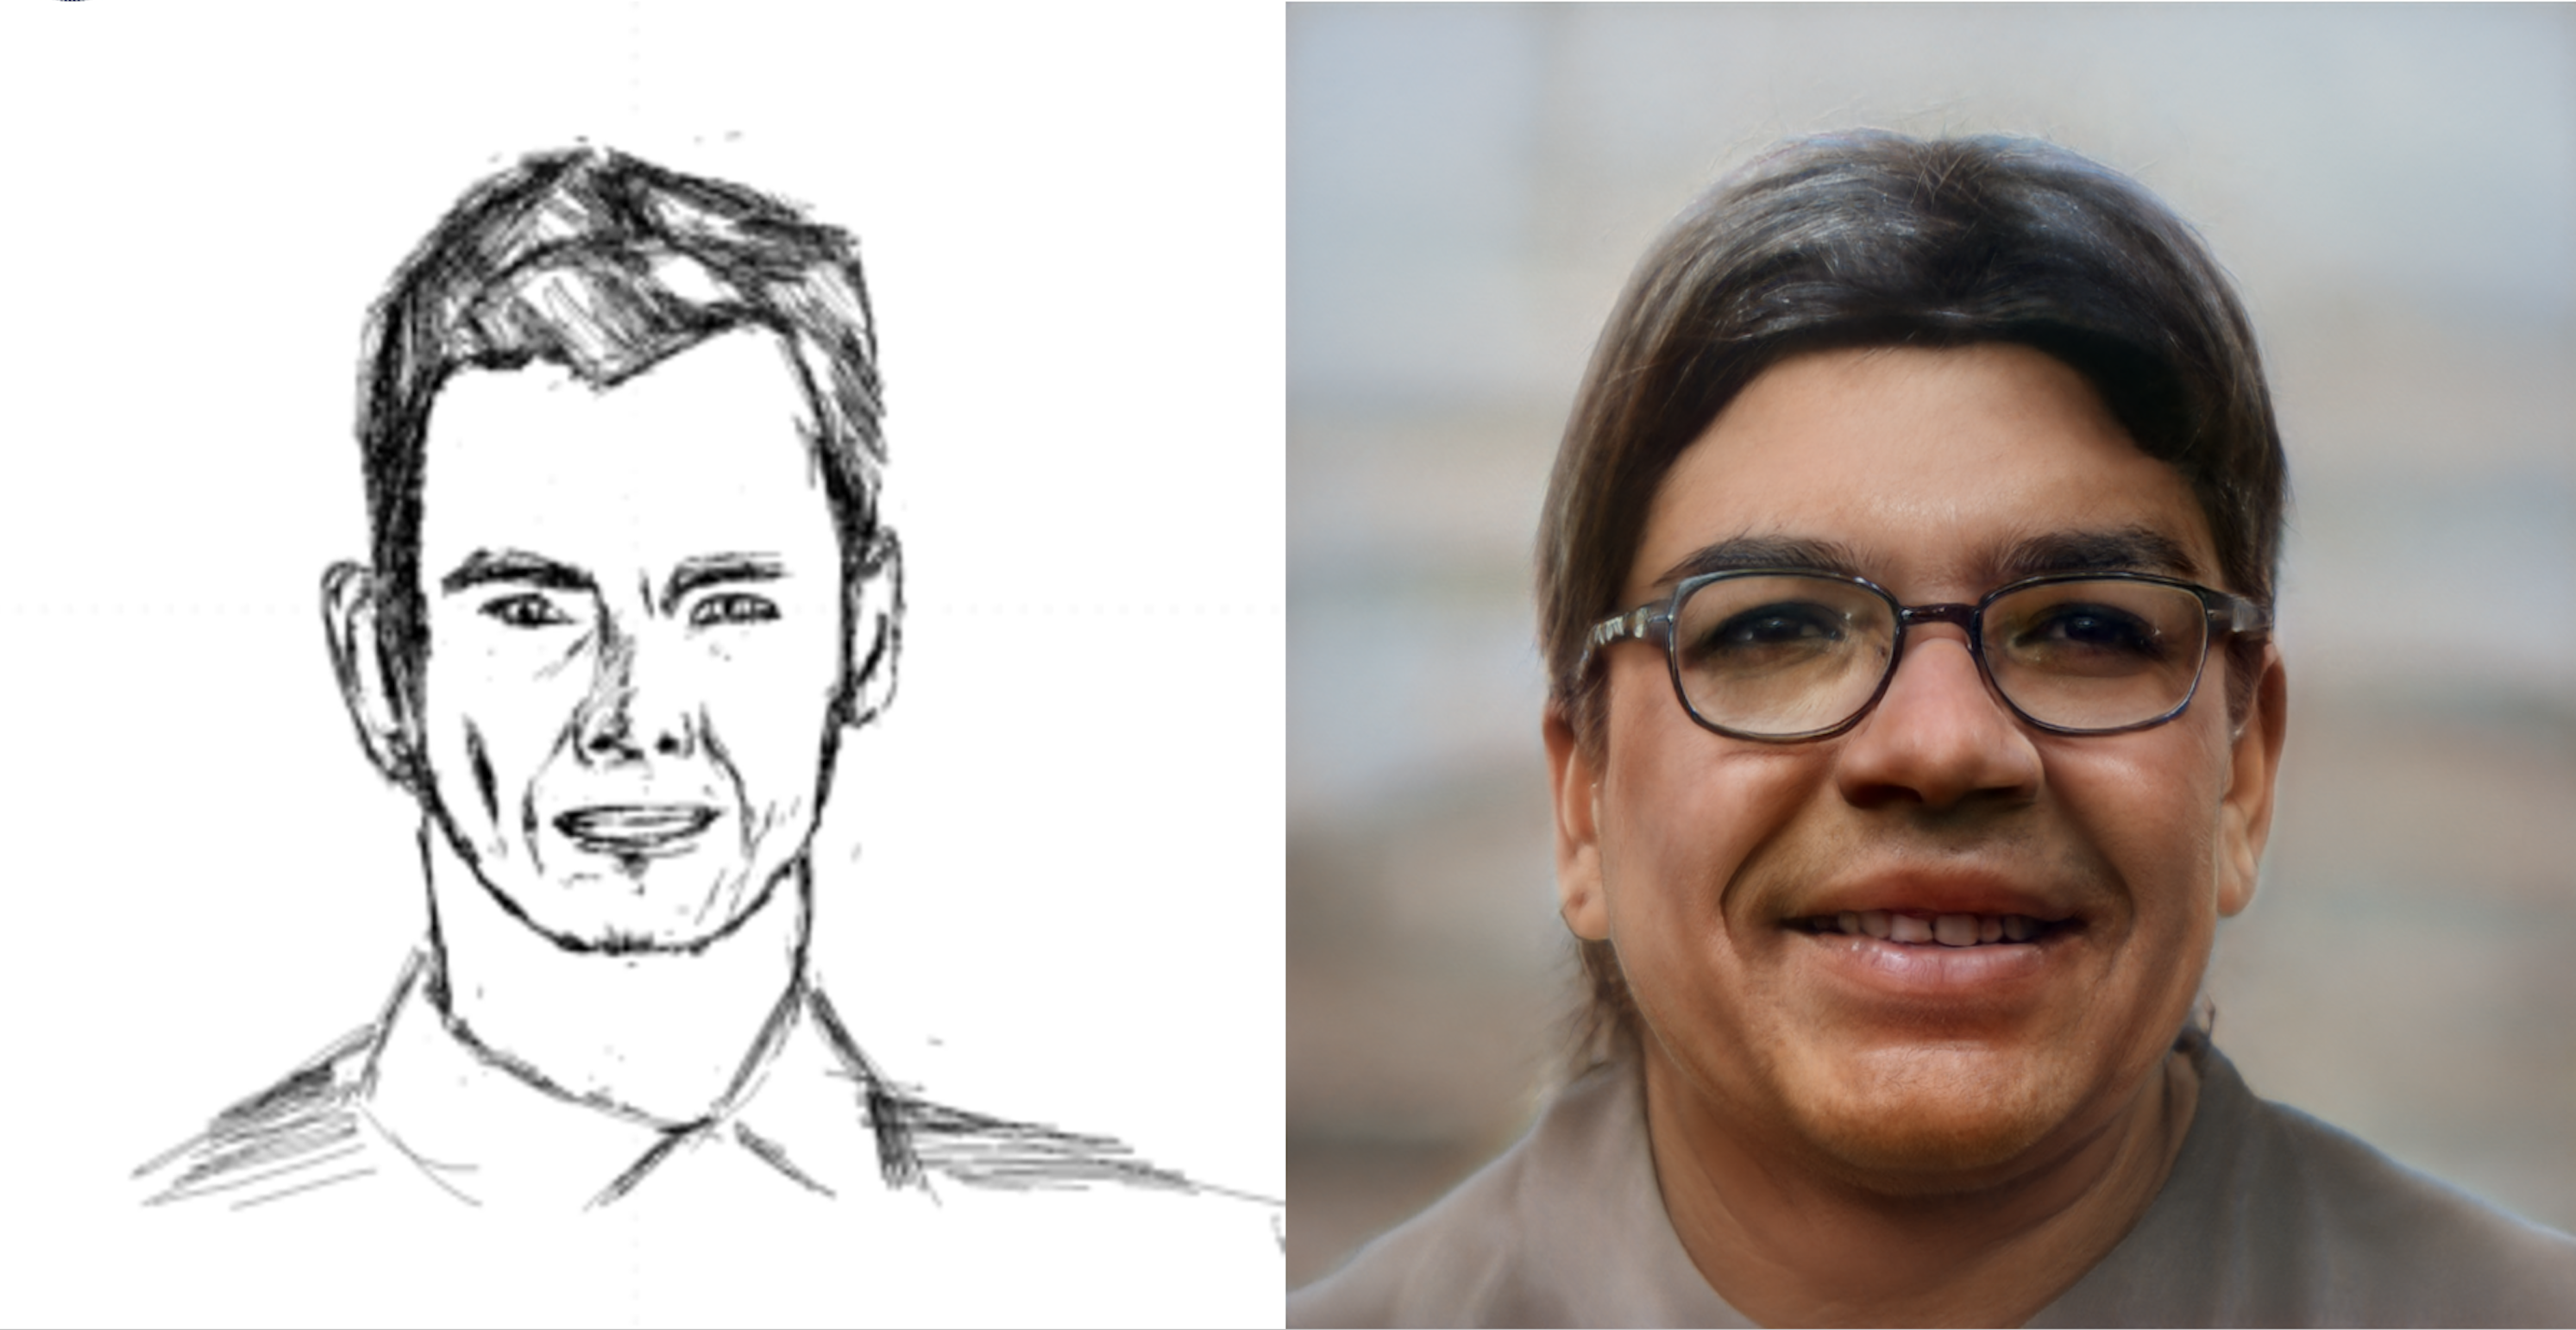
\includegraphics[scale=0.15]{figures/badResult1.png}
  \caption{Disappointing result generated from a sketch too small}
  \label{fig:disappointing sketch small}
\end{figure}

\noindent As illustrated in Fig.~\ref{fig:result thick pen}, the use of a pen too thick can have a negative effect on the generated images, for example it can generate unrealistic hair and colours. However, upon closer examination of the generated image, it can be observed that certain details of the original sketch are still present. 
\begin{figure}[htbp]
  \centering
  \includegraphics[scale=0.15]{figures/badResult.png}
  \caption{Result obtained from a sketch made with a thick pen}
  \label{fig:result thick pen}
\end{figure}
%

\noindent Impressive results can be achieved when talented people create the sketches. It is worth noting that the success of the generated image is highly dependent on the quality of the input sketch. Where the term “quality” is related to the dimension of the sketch and the pen's thickness.
Therefore, it is essential to carefully consider the conditions under which the sketch is created to obtain optimal results. An example of a very breathtaking result can be seen in Fig.~\ref{fig:impressive result}, while Fig.~\ref{fig:result simple sketch} depicts a straightforward input sketch and its corresponding generated image that exhibits noticeable similarity.
\begin{figure}[htbp]
  \centering
  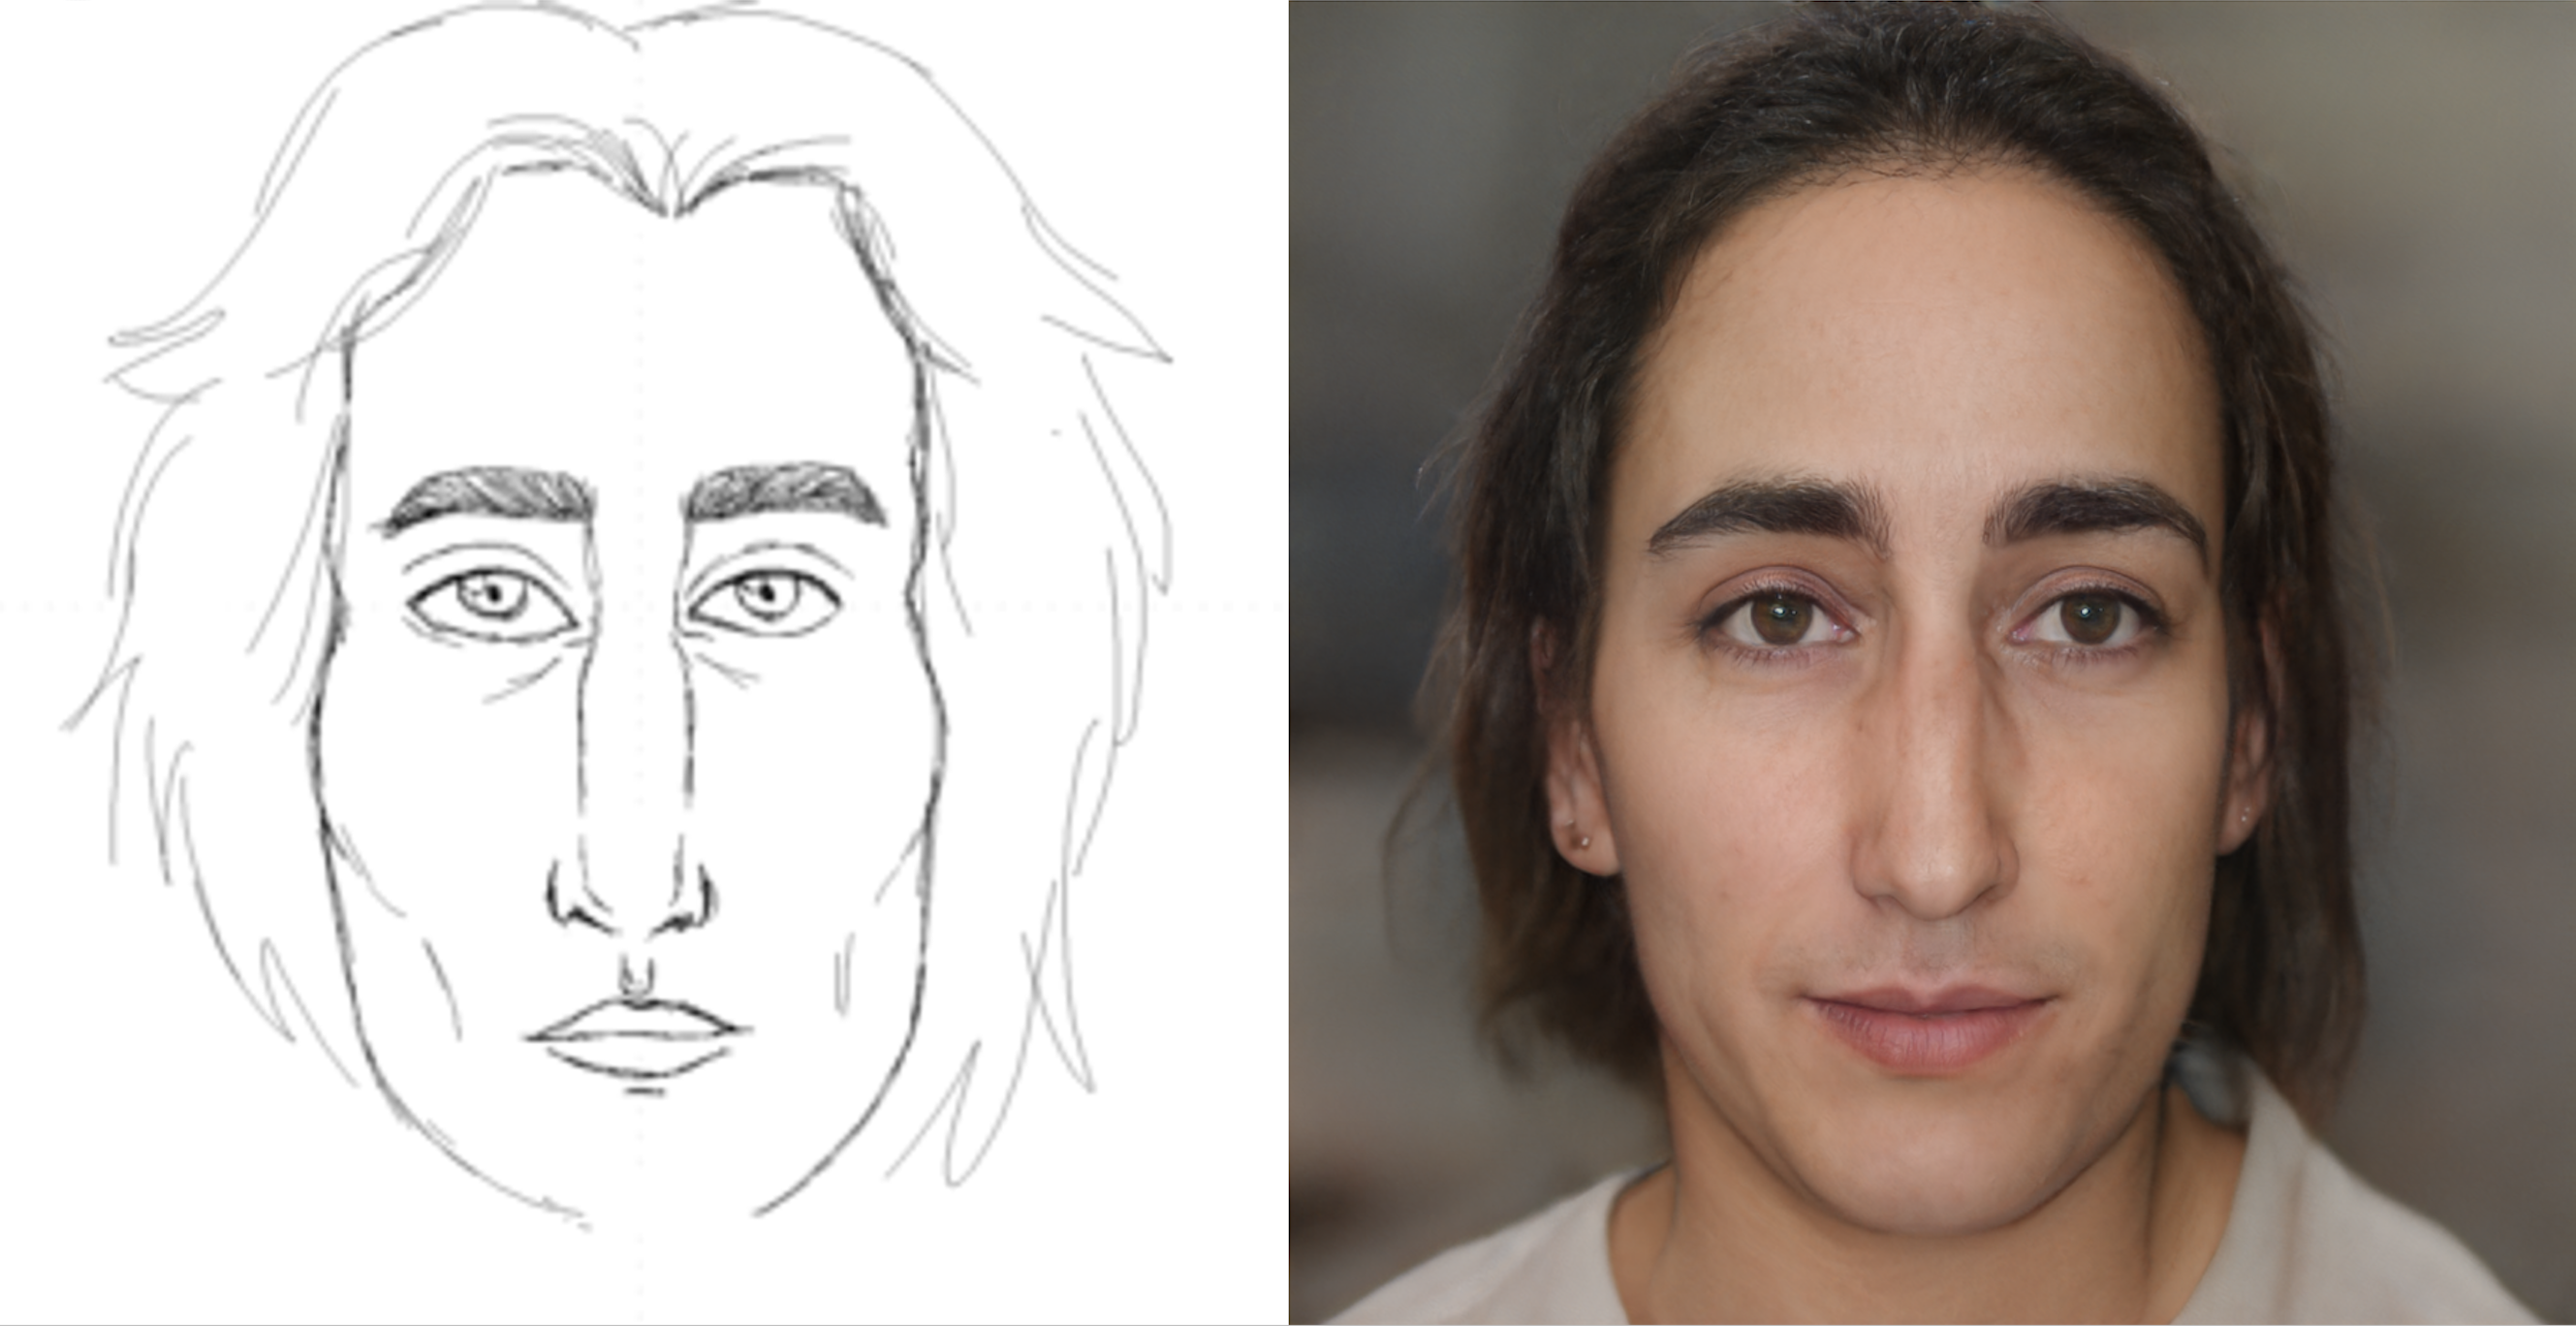
\includegraphics[scale=0.15]{figures/goodResult.png}
  \caption{Impressive result of an image generated from a sketch}
  \label{fig:impressive result}
\end{figure}
\begin{figure}[htbp]
  \centering
  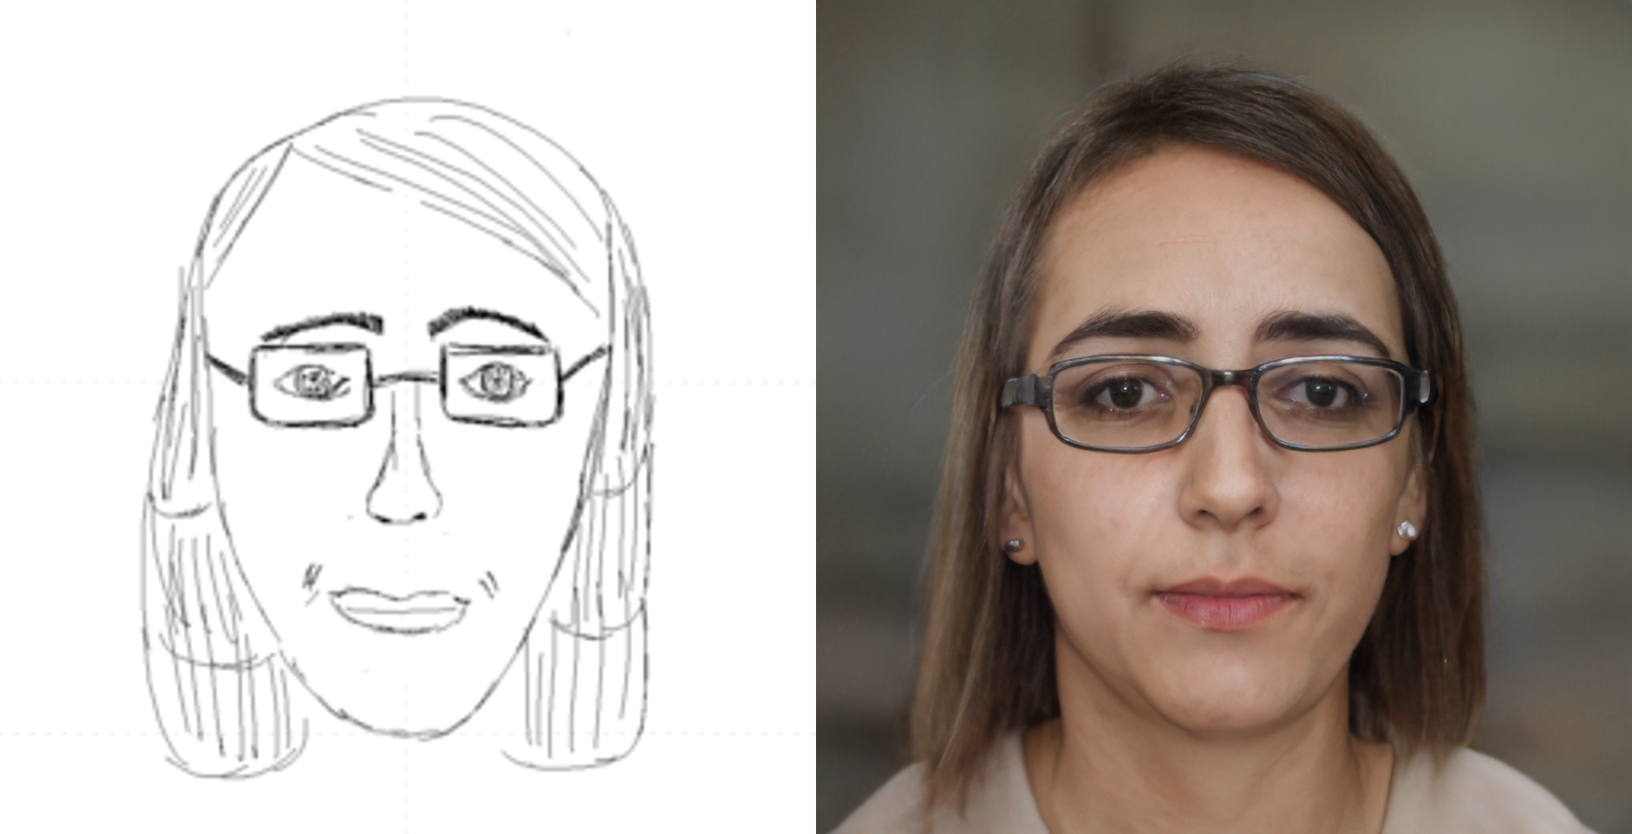
\includegraphics[scale=0.25]{figures/goodResult-simpleSketch.png}
  \caption{Result of an image generated from a simple sketch}
  \label{fig:result simple sketch}
\end{figure}
%

\noindent Given the diverse range of people who contributed to the sketch dataset, consisting of individuals with varying age groups and drawing abilities, it became necessary to filter out sketches that were unrealistic. Furthermore, some sketches displayed minor differences, as shown in Fig.~\ref{fig:similar sketches}, or only portrayed the outline of the face without any distinguishable feature (Fig.~\ref{fig:discarded images}).
\begin{figure}[htbp]
    \centering
    \subfloat[][\emph{ }]
    {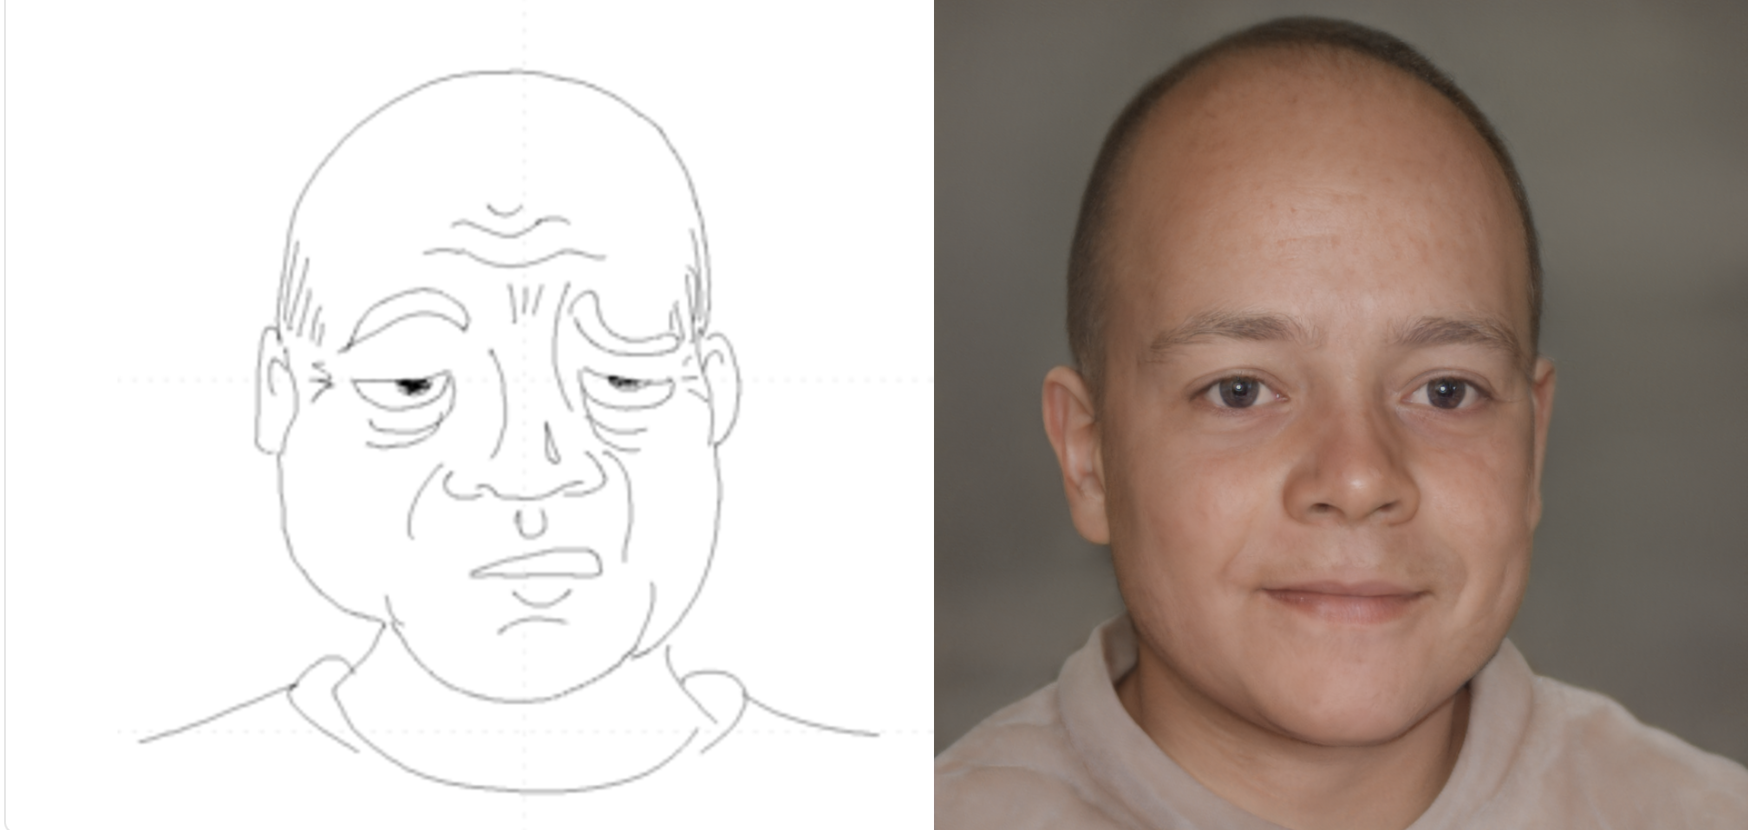
\includegraphics[width=.4\textwidth]{figures/similarSketch2.png}} \quad
    \subfloat[][\emph{}]
    {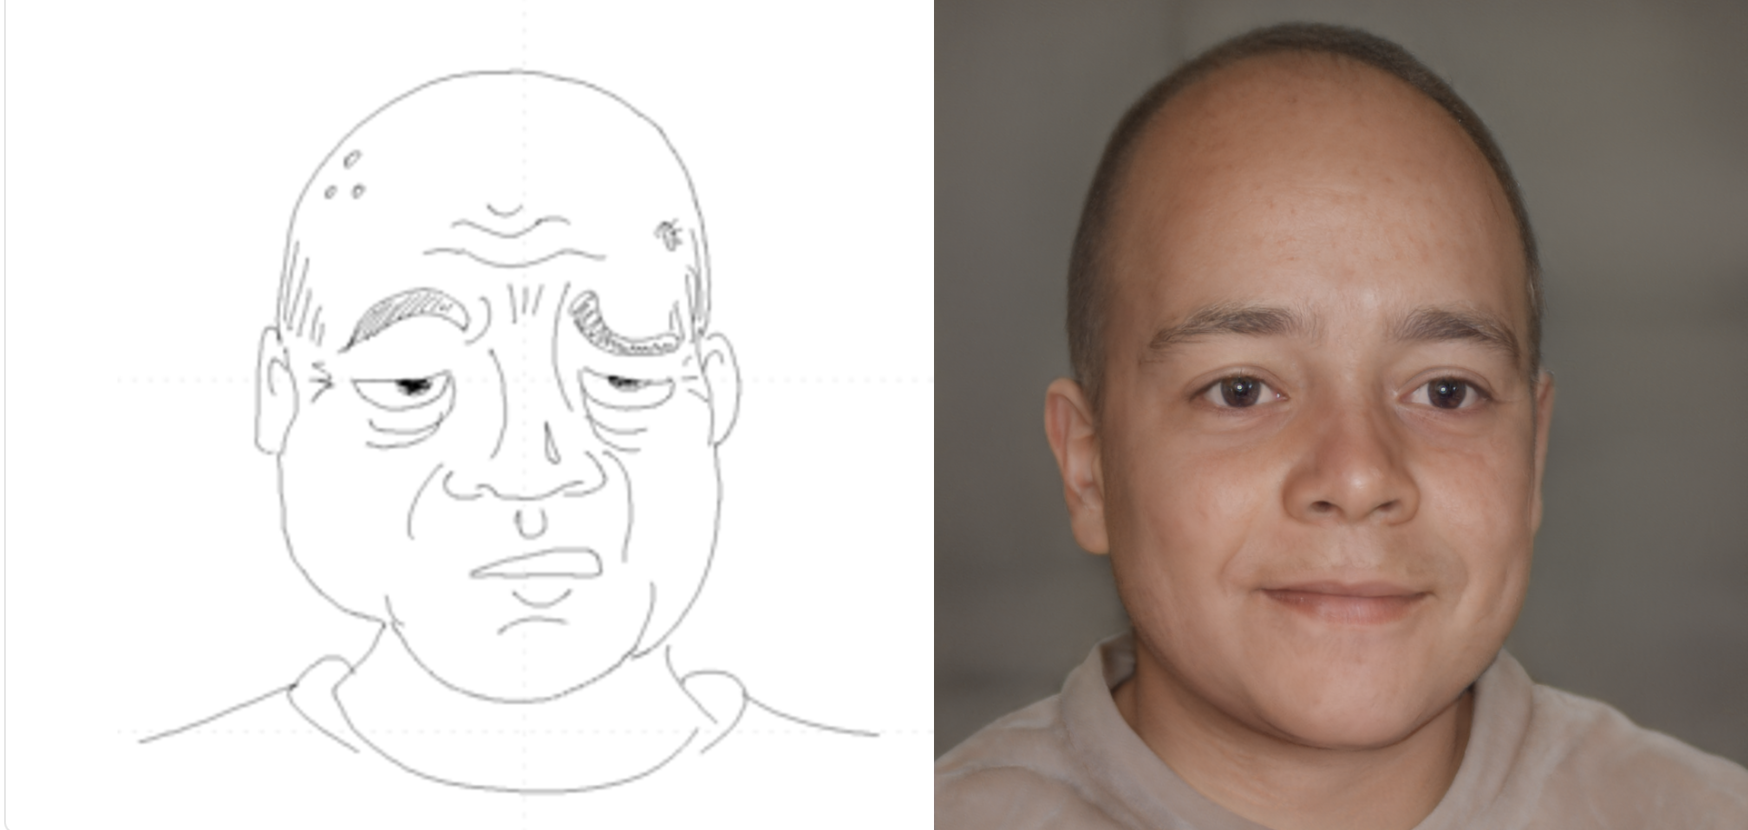
\includegraphics[width=.4\textwidth]{figures/similarSketch1.png}}
    \caption{Examples of two similar sketches}
    \label{fig:similar sketches}
\end{figure}
\begin{figure}[htbp]
    \centering
    \subfloat[][\emph{Empty sketch}]
    {
\includegraphics[width=.4\textwidth]{figures/emptySketch.png}} \quad
    \subfloat[][\emph{Sketch with just the contour of the face}]
    {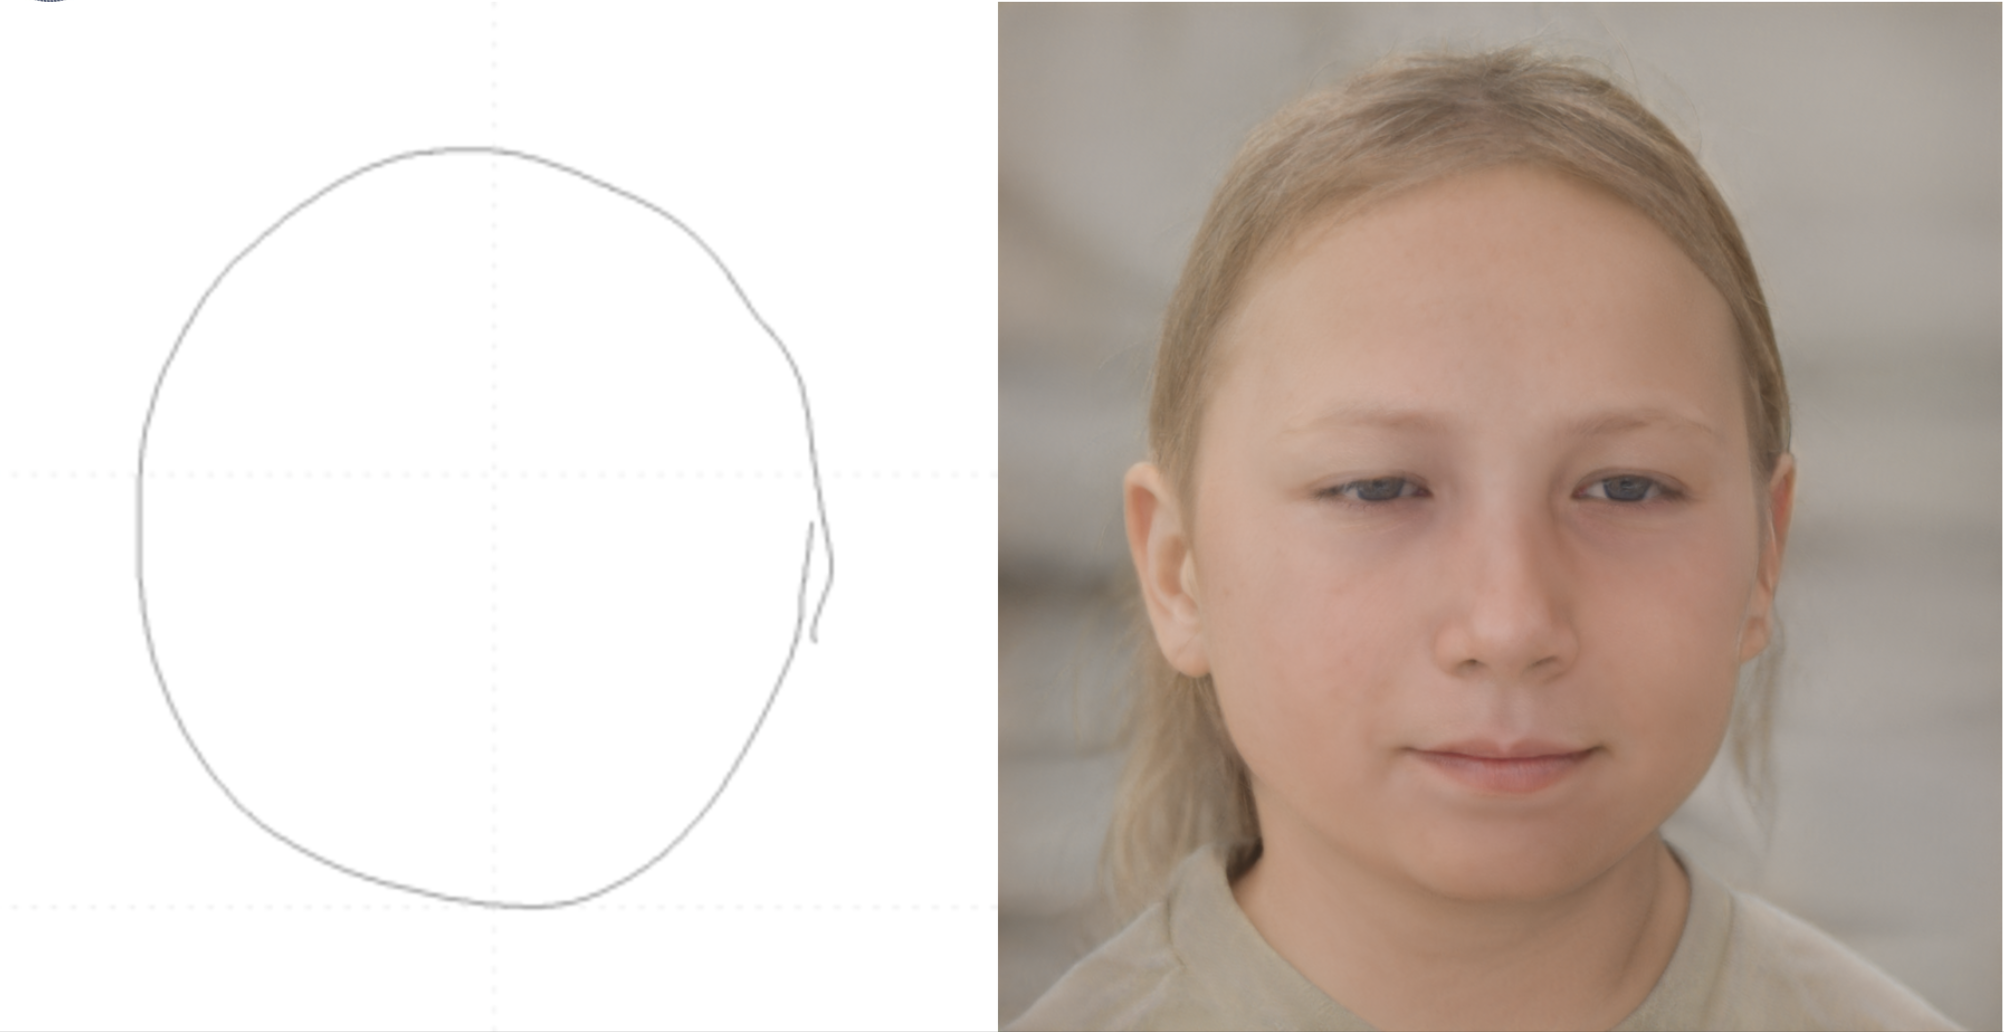
\includegraphics[width=.4\textwidth]{figures/sketchOnlyContour.png}}\\
    \subfloat[][\emph{Sketch done with a thick pen}]
    {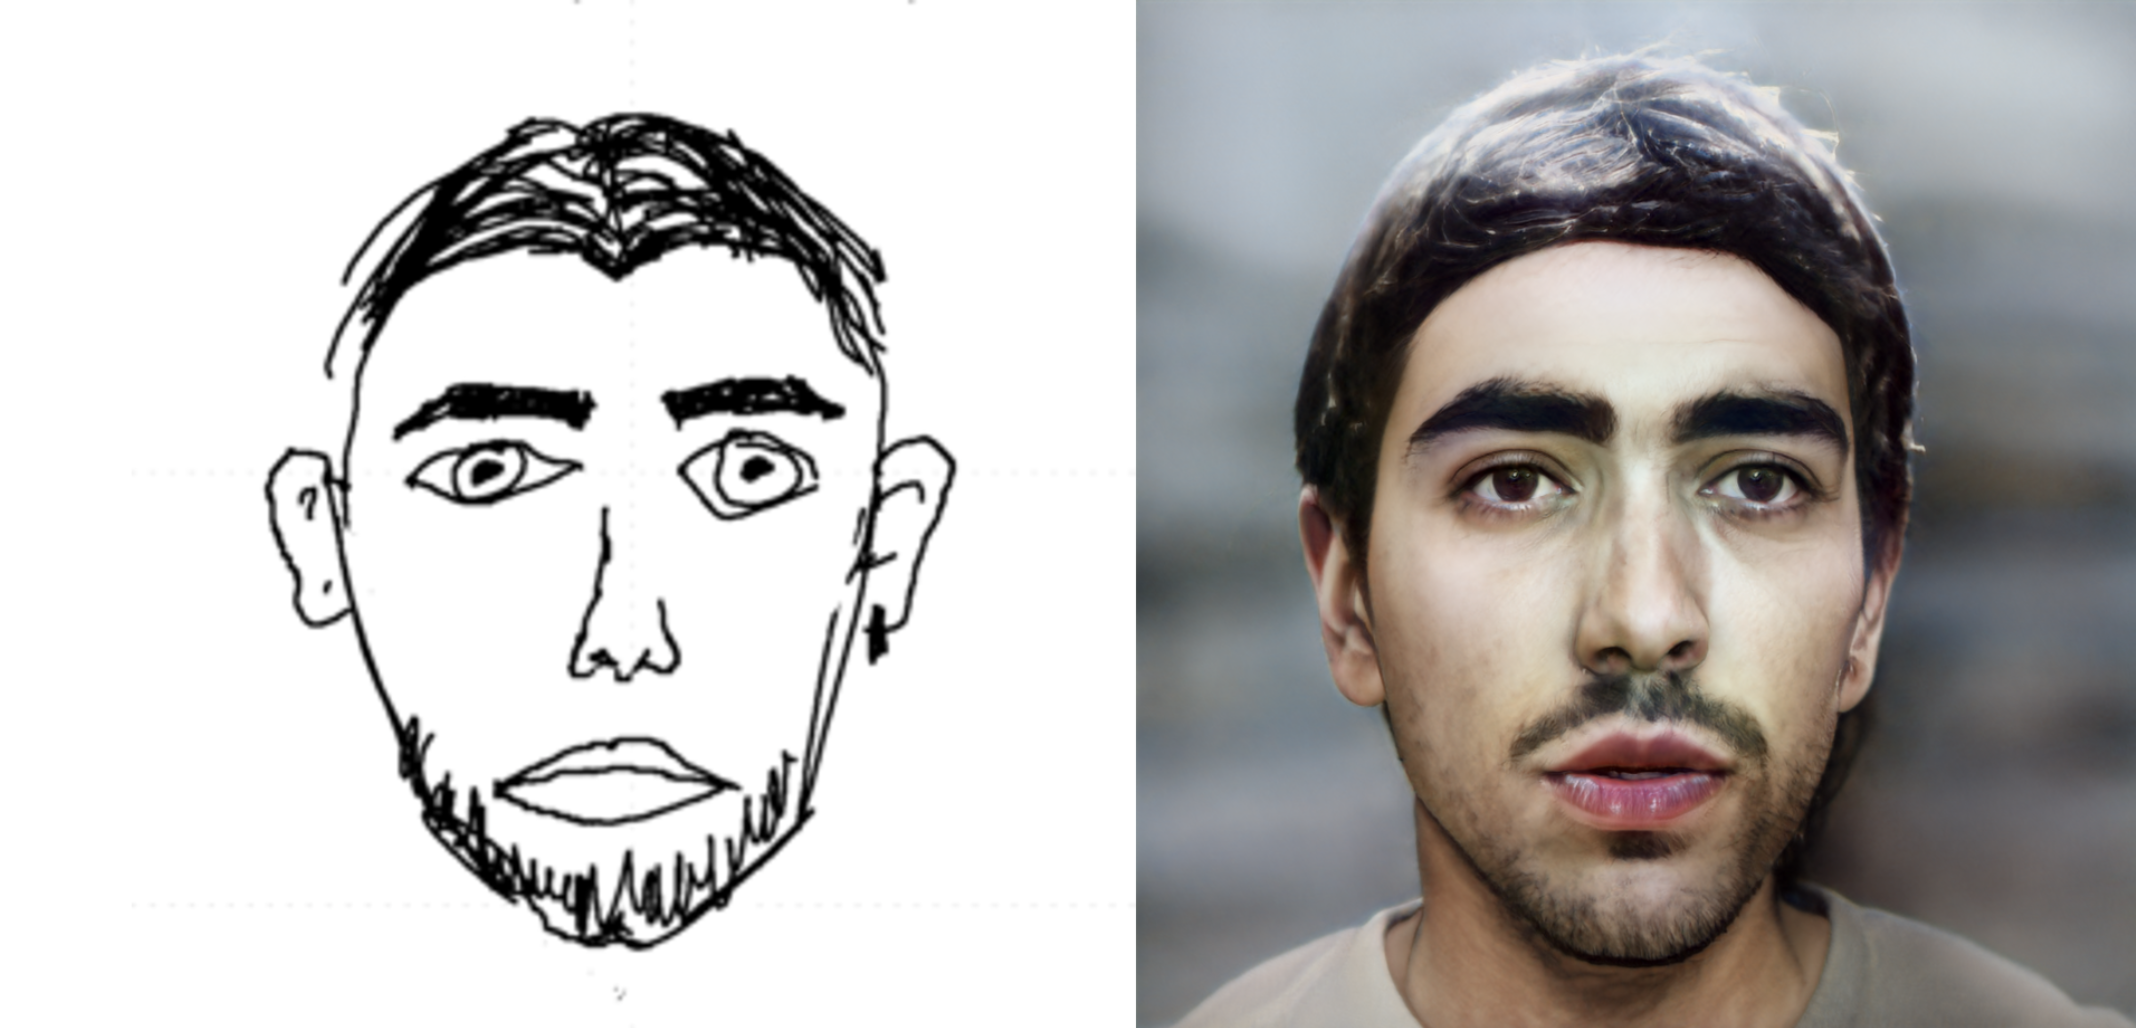
\includegraphics[width=.4\textwidth]{figures/thickPenSketch.png}}
    \caption{Examples of discarder images}
    \label{fig:discarded images}
\end{figure}

\noindent Therefore, the initial set of sketches was manually processed to remove such sketches, leaving only the more realistic ones. Subsequently, the remaining images underwent further analysis, and the poorest sketches were discarded. Finally, the xCos metric was applied to the filtered dataset to identify the most similar images to the sketches.


\noindent The survey was built in such a way that \num{5} random images out of the \num{20} are displayed. The survey's participants were instructed to choose the image that in their opinion had inspired the realisation of the sketch. An example of how the images are displayed in the survey is shown in Fig.~\ref{fig:survey images}.
\begin{figure}[htbp]
    \centering
    \subfloat[][\emph{ }]
    {
\includegraphics[width=.8\textwidth]{figures/survey1.png}} \quad
    \subfloat[][\emph{}]
    {
\includegraphics[width=.8\textwidth]{figures/survey2.png}}
    \caption{Examples of the structure of the survey}
    \label{fig:survey images}
\end{figure}
%

\subsection{Survey's results}
\label{sec:survey results}
Out of the \num{202} responses collected from the survey,  only \num{155} were considered for the analysis because the remaining \num{47} came from people try to complete the survey a second time.


\noindent Figure~\ref{fig:bar plot with correct/incorrect responses} (a) and (b) provide an overview of the results obtained from the survey. The figure displays the total number of correct and incorrect responses for each sketch, indicated by green and red bars, respectively. The sketches are labelled on the x-axis.

\begin{figure}[!b]
  \centering
  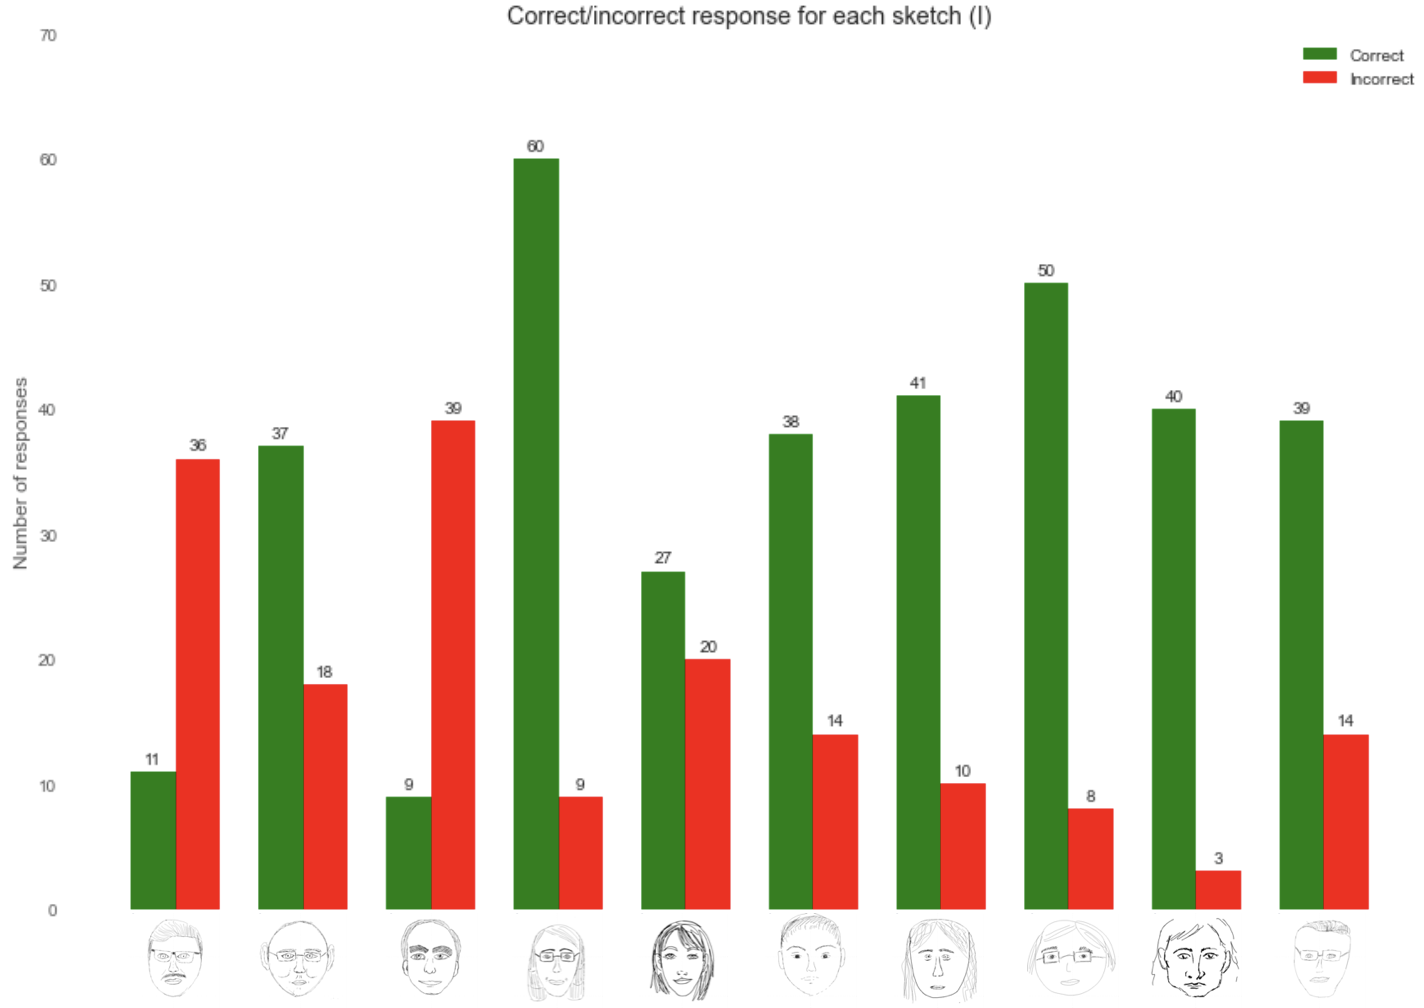
\includegraphics[width=1\textwidth]{figures/RISULTATI/correctIncorrectResponses-1.png}
  \caption{Results for the first \num{10} sketches (a).}
  \label{fig:bar plot with correct/incorrect responses}
\end{figure}

\begin{figure}[ht]
  \ContinuedFloat
  \centering
  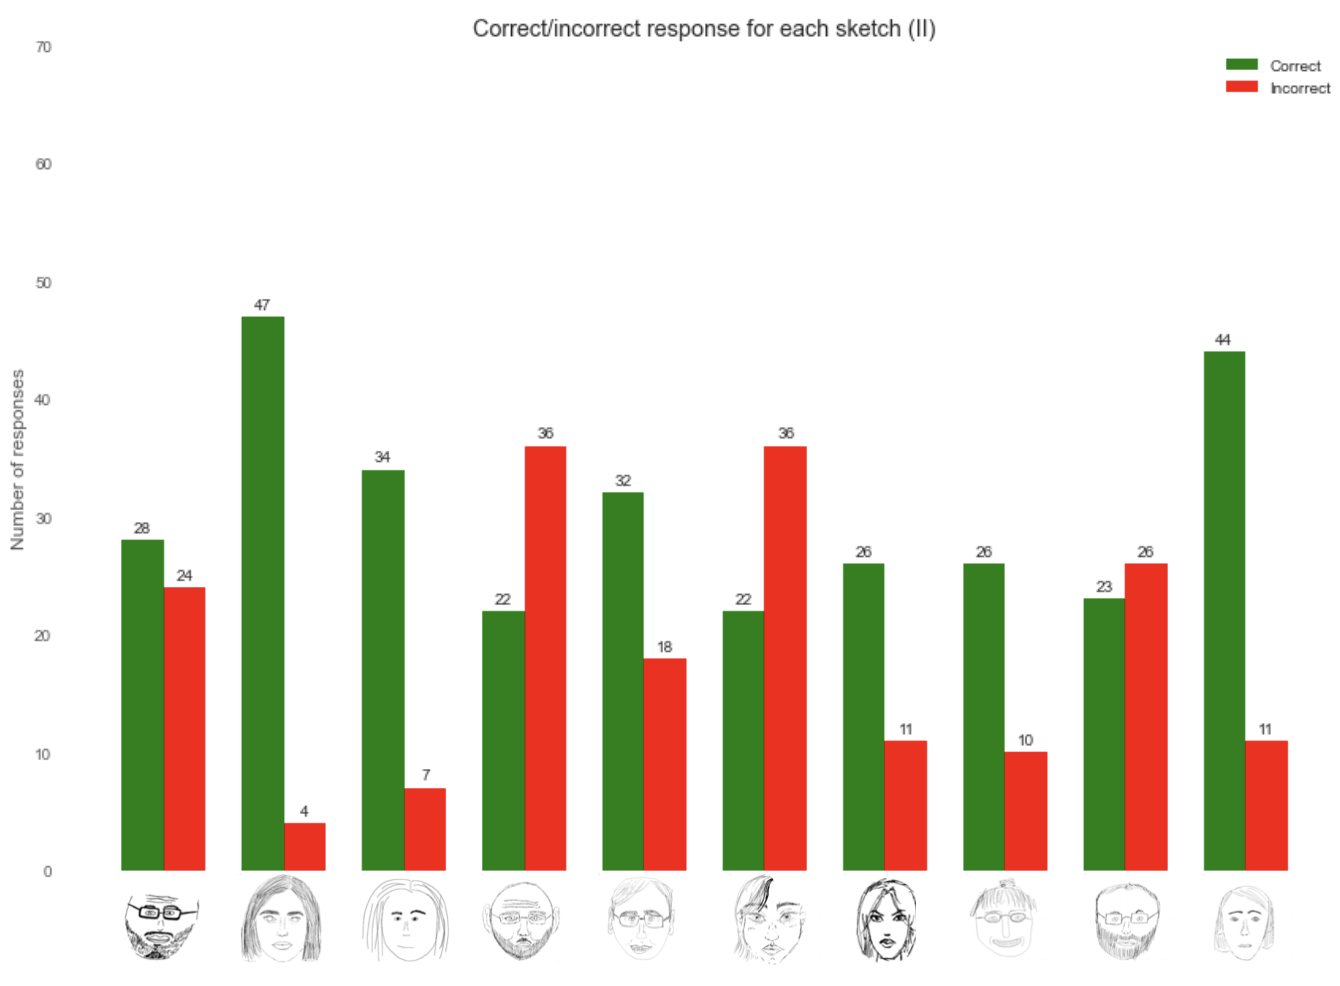
\includegraphics[width=1\textwidth]{figures/RISULTATI/correctIncorrectResponses-2.png}
  \caption{Results for the second \num{10} sketches (b).}
  \label{fig:bar plot with correct/incorrect responses}
\end{figure}

%\begin{figure}[htbp]
% \centering
%    \subfloat[][\emph{Results for the first \num{10} sketches}]
%    {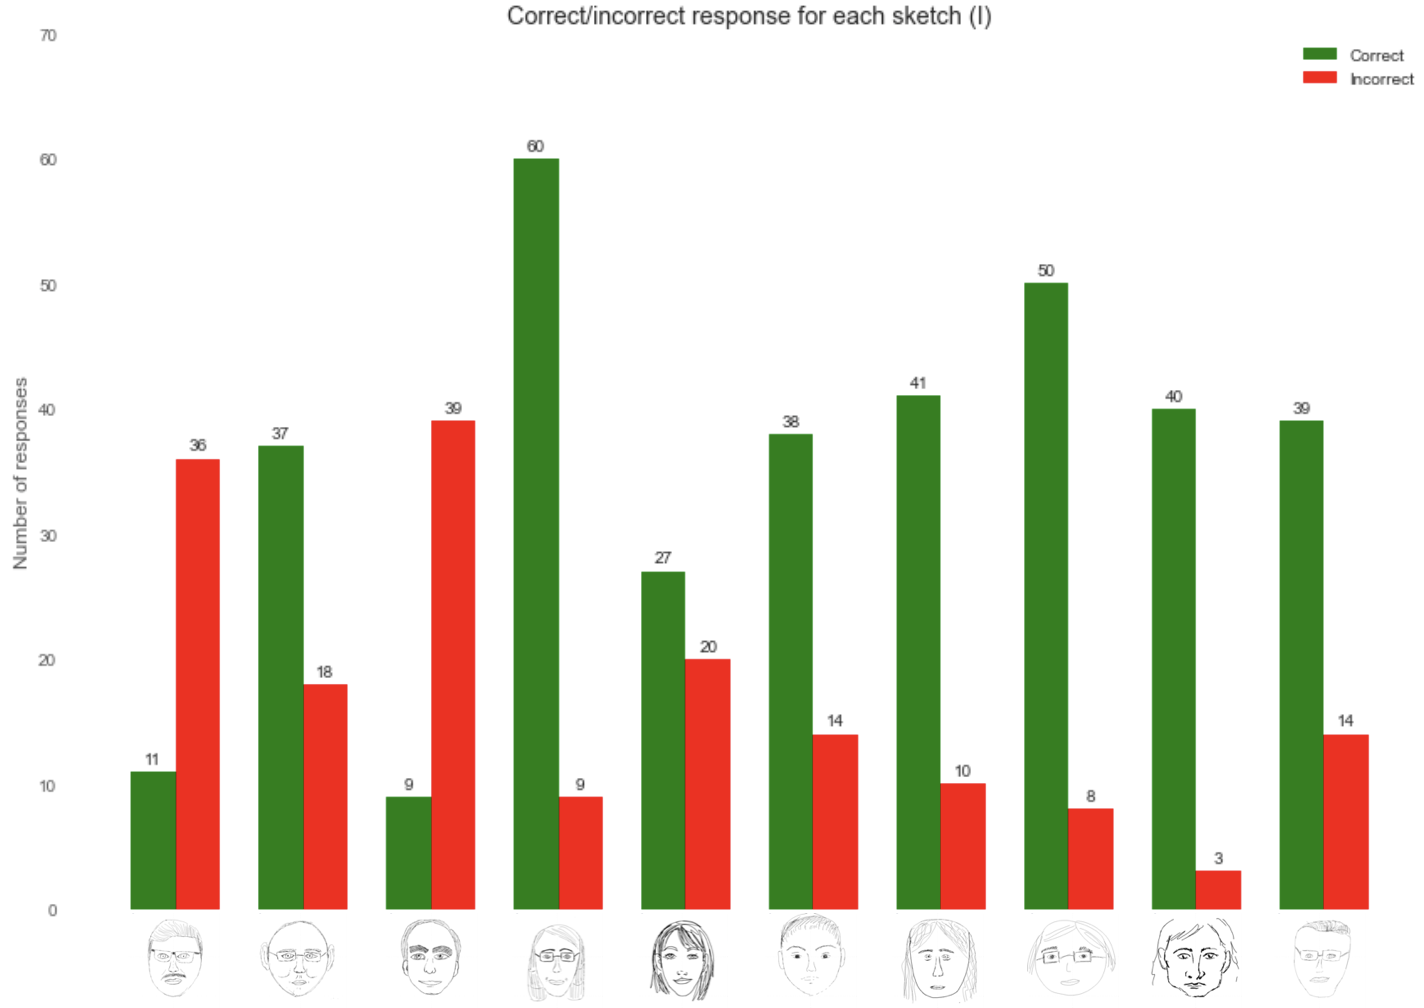
\includegraphics[width=.8\textwidth]{figures/RISULTATI/correctIncorrectResponses-1.png}} \\
%    \subfloat[][\emph{Results for the second \num{10} sketches}]
%    {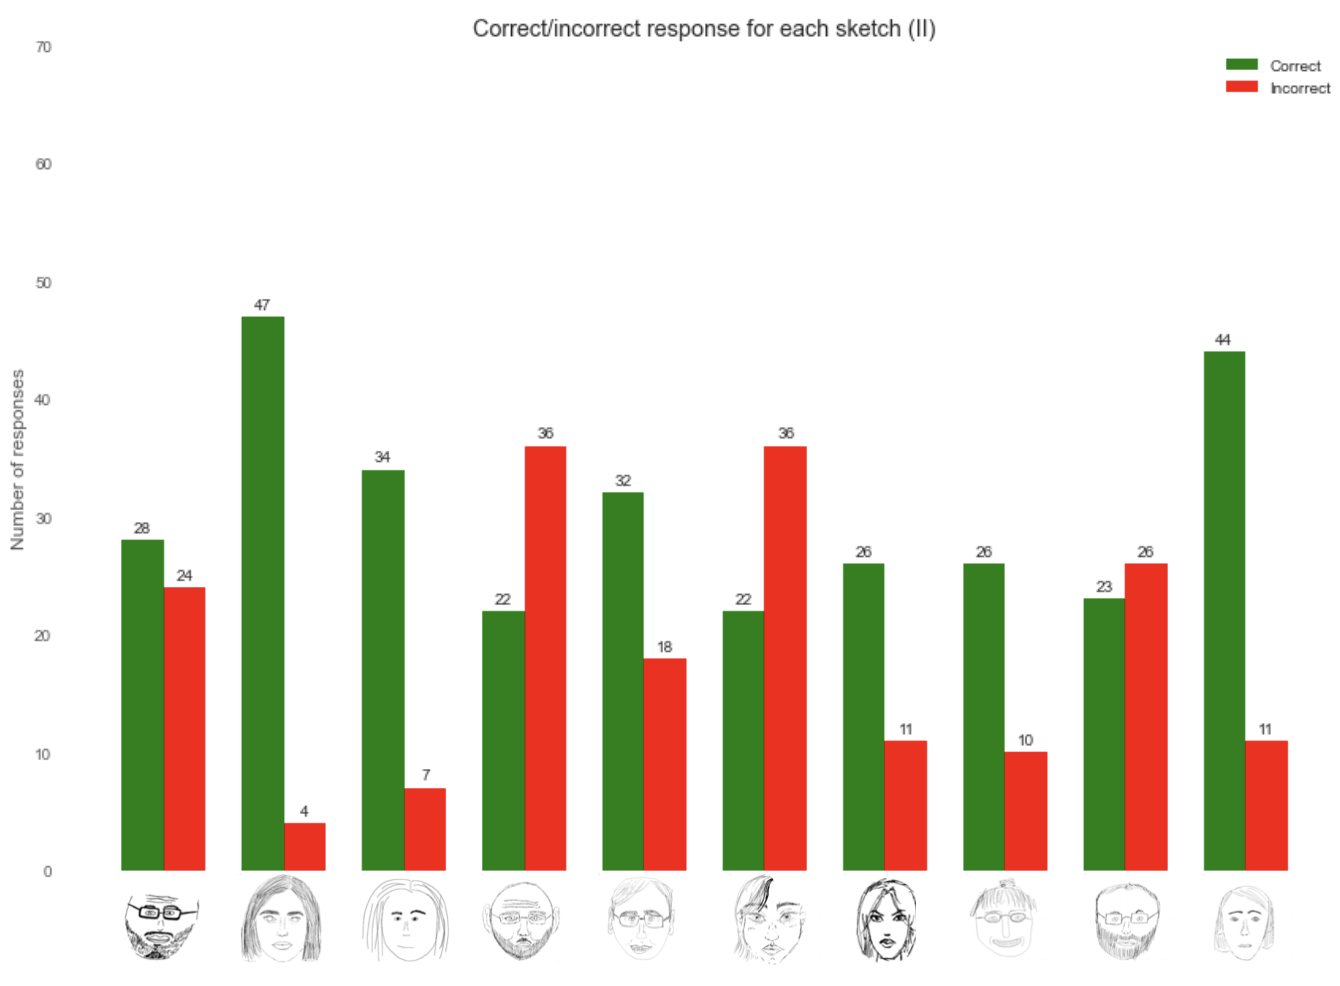
\includegraphics[width=.8\textwidth]{figures/RISULTATI/correctIncorrectResponses-2.png}}
%    \caption{}
%    \label{fig:bar plot with correct/incorrect responses}
%\end{figure}

   

\noindent Table~\ref{tab:responses summary} shows the percentage of correct responses and the average response time in seconds for each sketch in the survey.
\begin{table}[!ht]
\begin{center}
    \begin{tabular}{lcc}
    \textbf{SketchID} & \textbf{\% correct responses} & \textbf{average time (s)} \\
    0 & 23.4 \%  & 19.79 \\
    1 & 67.3 \%  & 14.13 \\
    2 & 18.8 \%  & 16.59\\
    3 & 87.0 \%  & 11.04 \\
    4 & 57.4 \%  & 14.08 \\
    5 & 73.1 \%  & 16.08 \\
    6 & 80.4 \%  & 14.52 \\
    7 & 86.2 \%  & 10.09 \\
    8 & 93.0 \%  & 12.48 \\
    9 & 73.6 \%  & 14.28 \\
    10 & 53.8 \%  & 21.19 \\
    11 & 92.2 \%  & 14.00 \\
    12 & 82.9 \%  & 19.45 \\
    13 & 37.9 \%  & 12.55 \\
    14 & 64.0 \%  & 13.78 \\
    15 & 37.9 \%  & 19.53 \\
    16 & 70.3 \%  & 15.43 \\
    17 & 72.2 \%  & 13.62 \\
    18 & 46.9 \%  & 18.90 \\
    19 & 80.0 \%  & 9.43 \\
    \hline
    \hline
    \textbf{Mean}: & 64.9 \% & 15.05
    \end{tabular}
     \caption{\label{tab:responses summary}Summary of the results obtained}
\end{center}
\end{table}
%
By looking at the column of the percentage of correct responses, two values stand out, namely the percentage of correct responses for the sketches with the IDs \num{2} and \num{8}. These two sketches have reported the smallest and the greatest percentage of correct responses, respectively.\\ 
The sketch with ID \num{2} can be seen in Fig.~\ref{fig:result sketch with greatest numb of incorrect}, where in Fig~\ref{fig:result sketch with greatest numb of incorrect}(a) each bar represents the number of responses obtained for each image. The third image in the plot obtained the highest number of responses, which may be attributed to the thick eyebrows depicted in the sketch, and also because the drawing gives the impression that it is a male subject.
The average time spent for each image is shown in Figure~\ref{fig:result sketch with greatest numb of incorrect}(b).
\begin{figure}[!ht]
    \centering
    \subfloat[][\emph{ }]
    {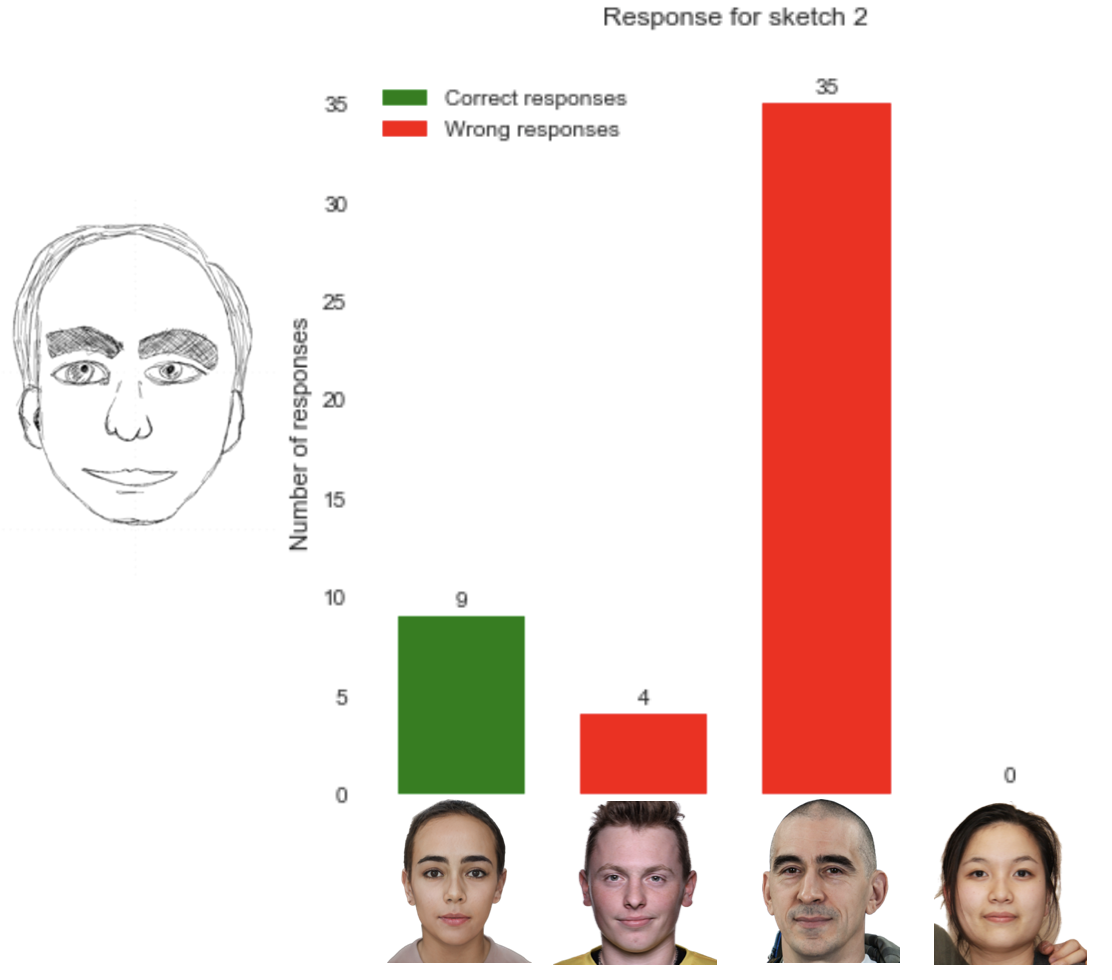
\includegraphics[width=.55\textwidth]{figures/RISULTATI/sketch2Responses.png}} \quad
    \subfloat[][\emph{}]
    {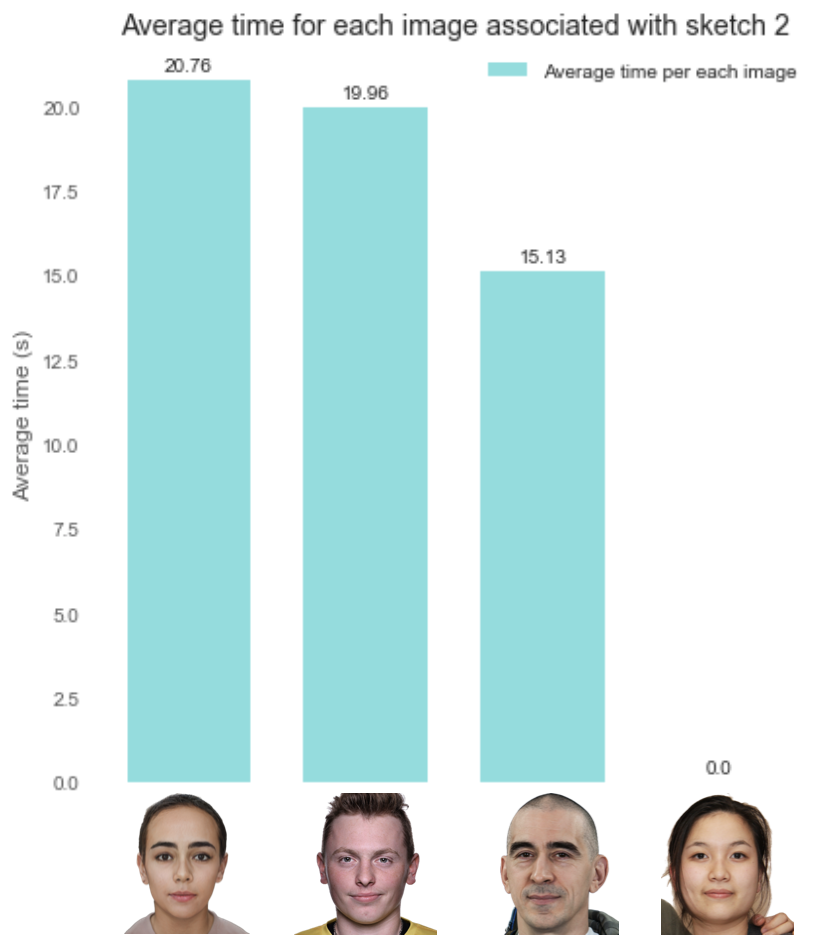
\includegraphics[width=.42\textwidth]{figures/RISULTATI/sketch2-time.png}}
    \caption{Sketch with the greatest percentage of incorrect responses}
    \label{fig:result sketch with greatest numb of incorrect}
\end{figure}

%
\noindent The results obtained for the sketch with ID \num{8} are shown in Fig.~\ref{fig:result sketch with greatest numb of correct}, where it can be observed that this sketch obtained the highest number of correct responses, most likely because the correct image was easily identifiable.

\begin{figure}[!ht]
    \centering
    \subfloat[][\emph{ }]
    {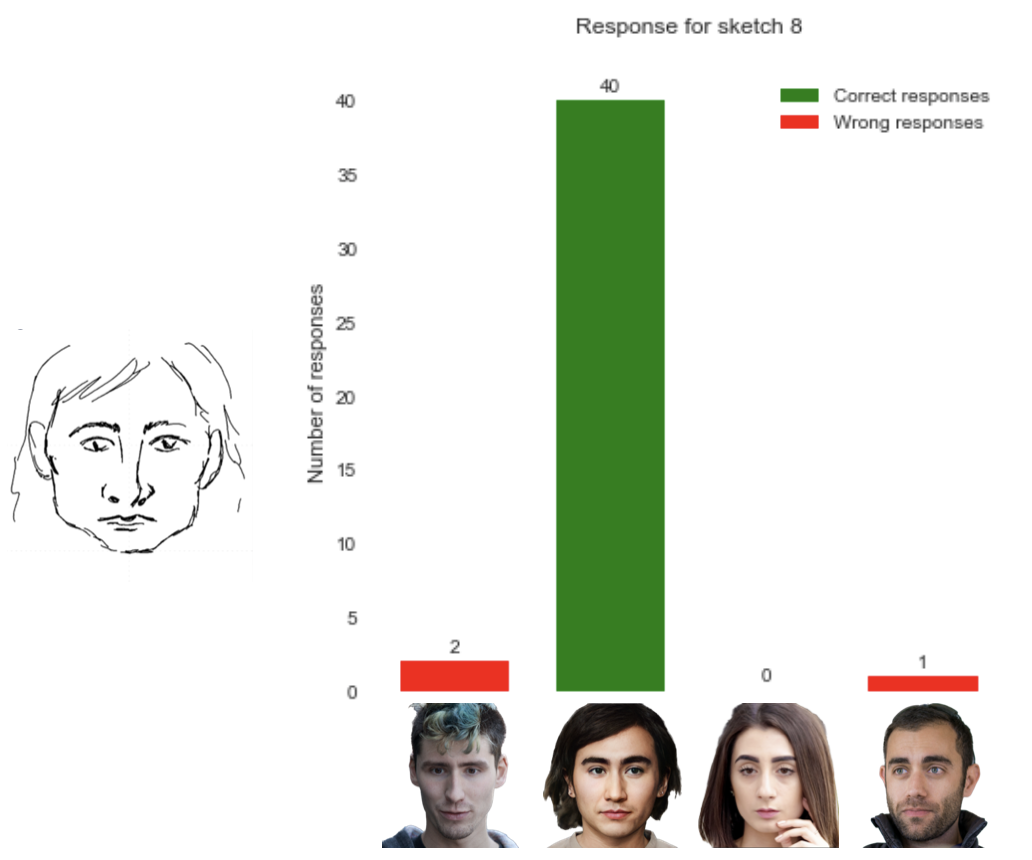
\includegraphics[width=.55\textwidth]{figures/RISULTATI/sketch8Responses.png}} \quad
    \subfloat[][\emph{}]
    {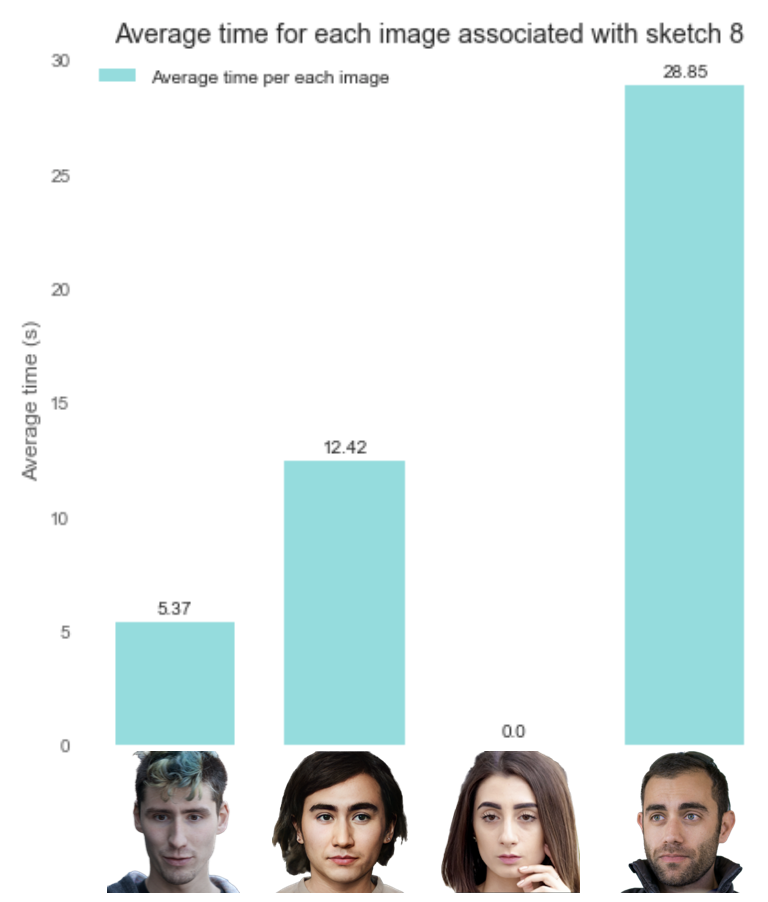
\includegraphics[width=.42\textwidth]{figures/RISULTATI/sketch8-time.png}}
    \caption{Sketch with the greatest percentage of correct responses}
    \label{fig:result sketch with greatest numb of correct}
\end{figure}

%
\noindent Looking at the average time, for almost all the images the time taken to choose a response is the same, exception made for sketch \num{19} and \num{10} that respectively obtained a lower and higher value than average time. In Figure~\ref{fig:result sketch with lowest average time}, the number of correct/incorrect responses and the average time for each similar image associated to sketch \num{19} are shown, and the same information are represented in Fig.~\ref{fig:result sketch with highest average time} for sketch \num{10}.\\
\begin{figure}[!ht]
    \centering
    \subfloat[][\emph{ }]
    {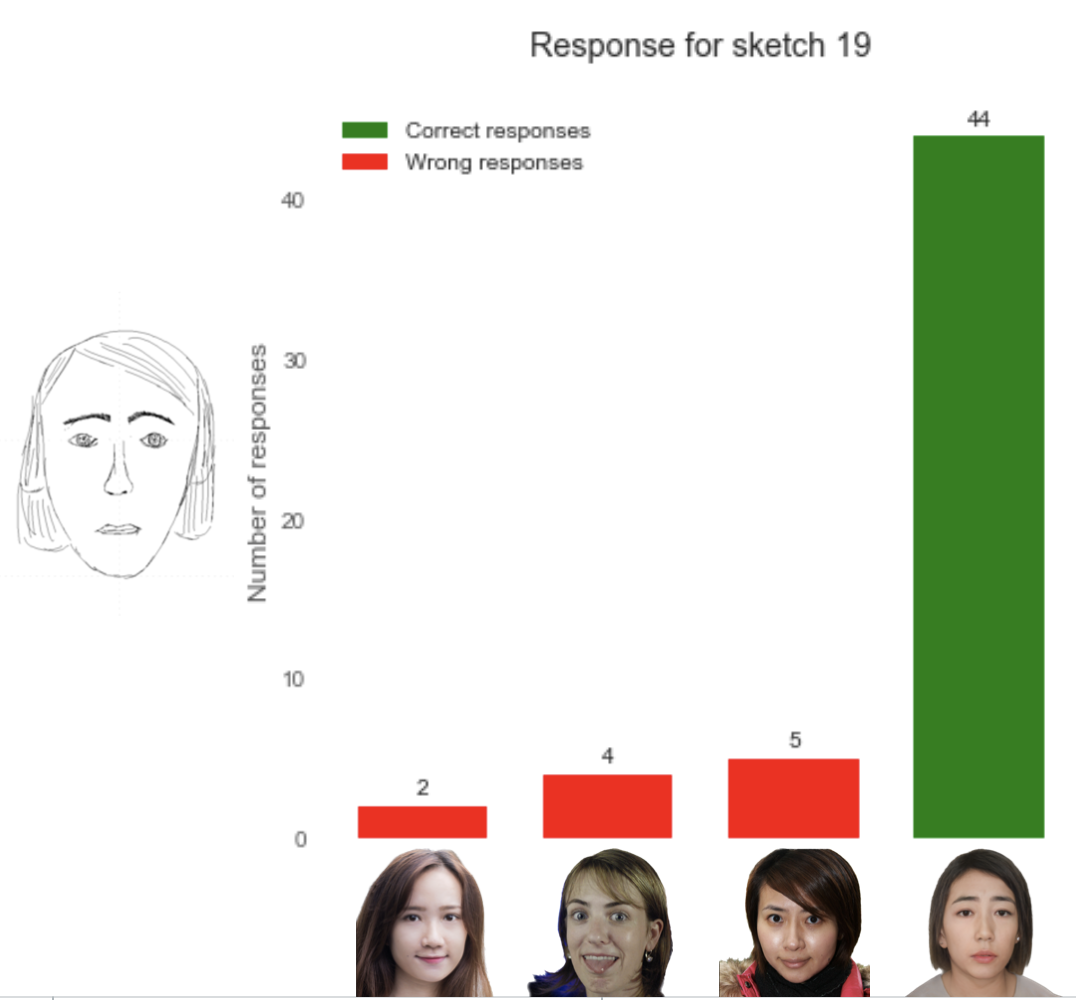
\includegraphics[width=.55\textwidth]{figures/RISULTATI/sketch19Responses.png}} \quad
    \subfloat[][\emph{}]
    {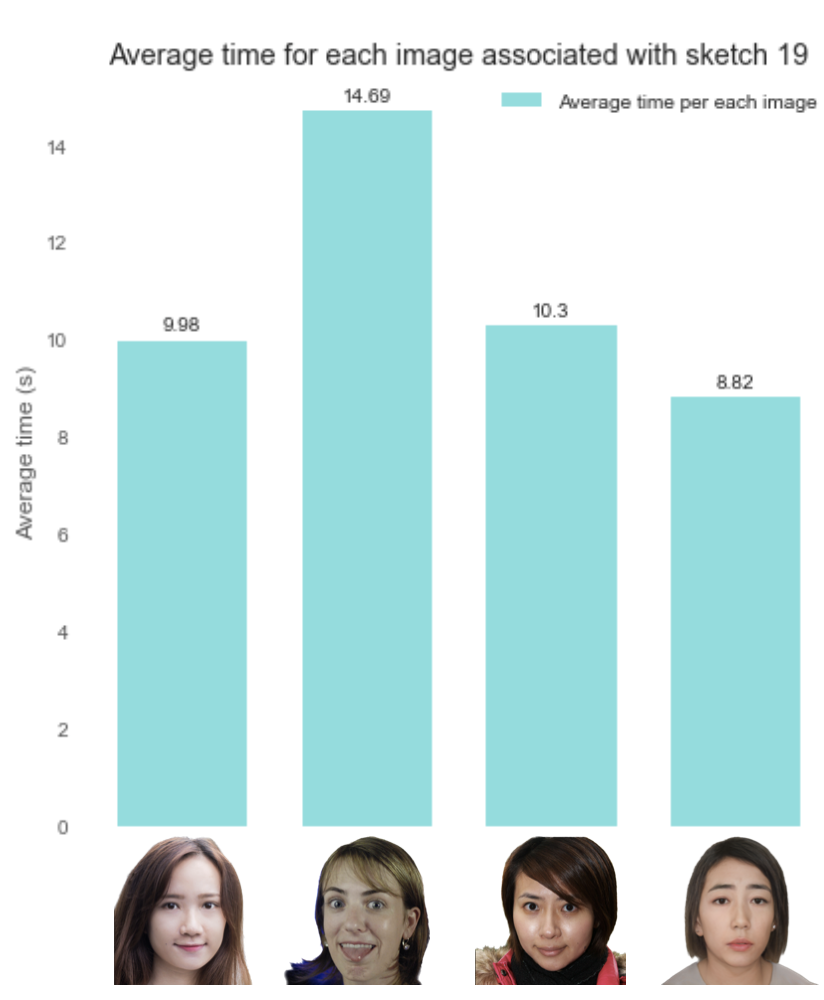
\includegraphics[width=.42\textwidth]{figures/RISULTATI/sketch19-time.png}}
    \caption{Sketch with the lowest average time}
    \label{fig:result sketch with lowest average time}
\end{figure}
\begin{figure}[!ht]
    \centering
    \subfloat[][\emph{ }]
    {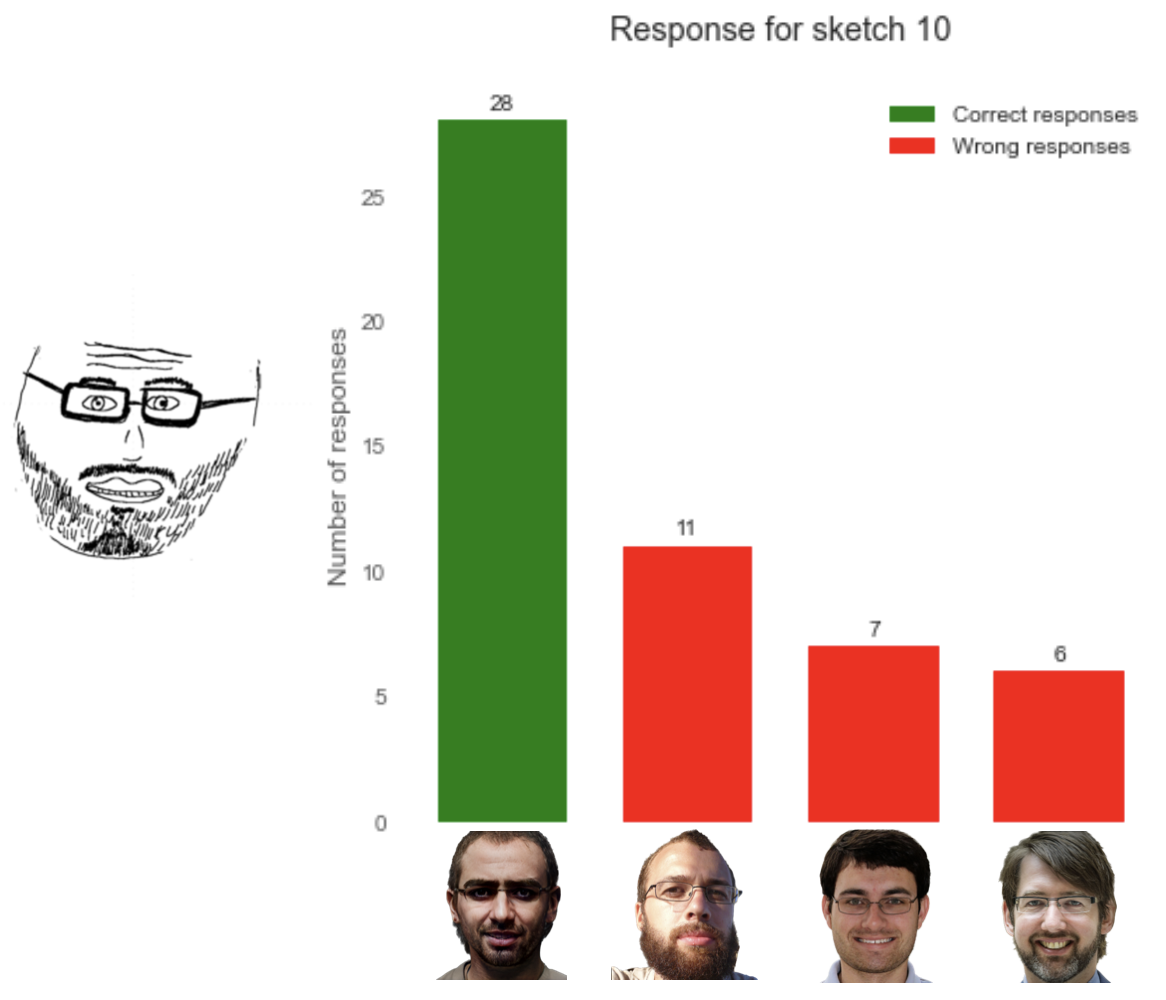
\includegraphics[width=.55\textwidth]{figures/RISULTATI/sketch10Responses.png}} \quad
    \subfloat[][\emph{}]
    {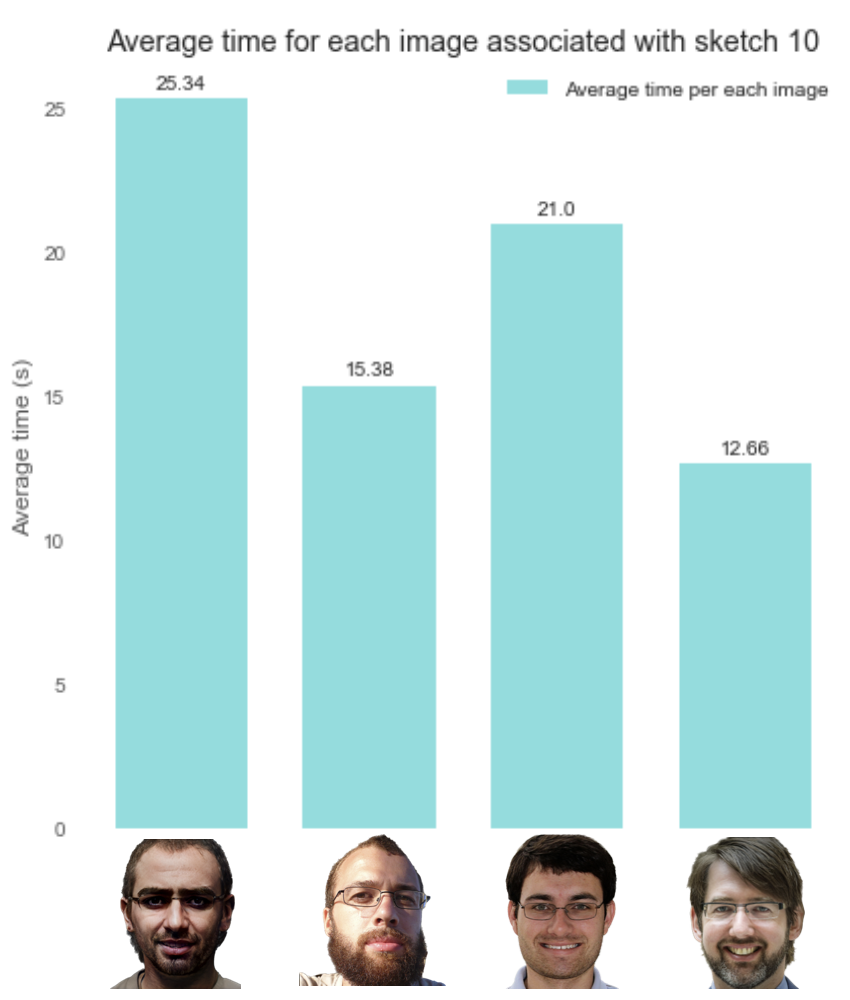
\includegraphics[width=.42\textwidth]{figures/RISULTATI/sketch10-time.png}}
    \caption{Sketch with the highest average time}
    \label{fig:result sketch with highest average time}
\end{figure}

\noindent Before drawing any conclusions, it is of extreme importance to determine whether the proportion of correct answers is due to an actual understanding of the difference between the proposed images and people could actually determine which of the images was inspired by the sketch, rather than just guessing the correct answer. Therefore, the binomial test was performed, to calculate the likelihood of getting a certain number of successes, based on the assumption that the result was randomly obtained. The test essentially checks if the results are statistically significant or just due to random chance.

\noindent The null hypothesis considered in this test is that there is no significant difference between the observed proportion of success and the expected proportion of success by chance, while the p-value represents the probability of observing more extreme outcomes than the observed ones.
If the p-value is below a predetermined significance level, the null hypothesis is rejected, and it is concluded that the observed outcome is unlikely to be due to chance alone.

\noindent For each question in the survey there are four possible responses, but just one is correct, therefore the probability of guessing it correctly is \num{25}\%.
The significance value alpha is set to \num{0.05} for all tests. The null hypothesis for the test states that the proportion of correct answers is equal to \num{25}\%, while the alternative hypothesis was that the proportion was greater than \num{25}\%.

\noindent The results of the analysis, shown in Table~\ref{tab:binomial test results}, indicate that, for \num{18} out of the \num{20} questions, the p-value is less than alpha. This suggests that the percentage of correct responses is significantly higher than chance, meaning that it is unlikely that the correct responses are the result of random choices.
%
\begin{table}[!ht]
\begin{center}
    \begin{tabular}{lc}
    \textbf{SketchID} & \textbf{p-value}  \\
    0 & 0.65 \\
    1 & 0.00 \\
    2 & 0.88 \\
    3 & 0.00 \\
    4 & 0.00 \\
    5 & 0.00 \\
    6 & 0.00 \\
    7 & 0.00 \\
    8 & 0.00 \\
    9 & 0.00 \\
    10 & 0.00 \\
    11 & 0.00 \\
    12 & 0.00 \\
    13 & 0.02 \\
    14 & 0.00 \\
    15 & 0.02 \\
    16 & 0.00 \\
    17 & 0.00 \\
    18 & 0.00 \\
    19 & 0.00 \\
    \end{tabular}
     \caption{\label{tab:binomial test results}Results of the binomial test}
\end{center}
\end{table}

\noindent For the questions related to sketch \num{0} and \num{2}, the null hypothesis cannot be rejected, suggesting that the proportion of correct answer is not significantly different from chance. As can be noticed from Figure~\ref{fig:similar images sketch 0 and 2}, the images proposed for these sketches appear to be very similar, making the selection more challenging.
Overall, these findings suggest that the participants generally performed better than chance.

\noindent Furthermore, this statistical test was also performed on the overall results, considering the number of correct responses out of the total responses, that is \num{509} out of \num{775}. The p-value obtained in this case is \num{0.00}.\\
\begin{figure}[!ht]
    \centering
    \subfloat[][\emph{ }]
    {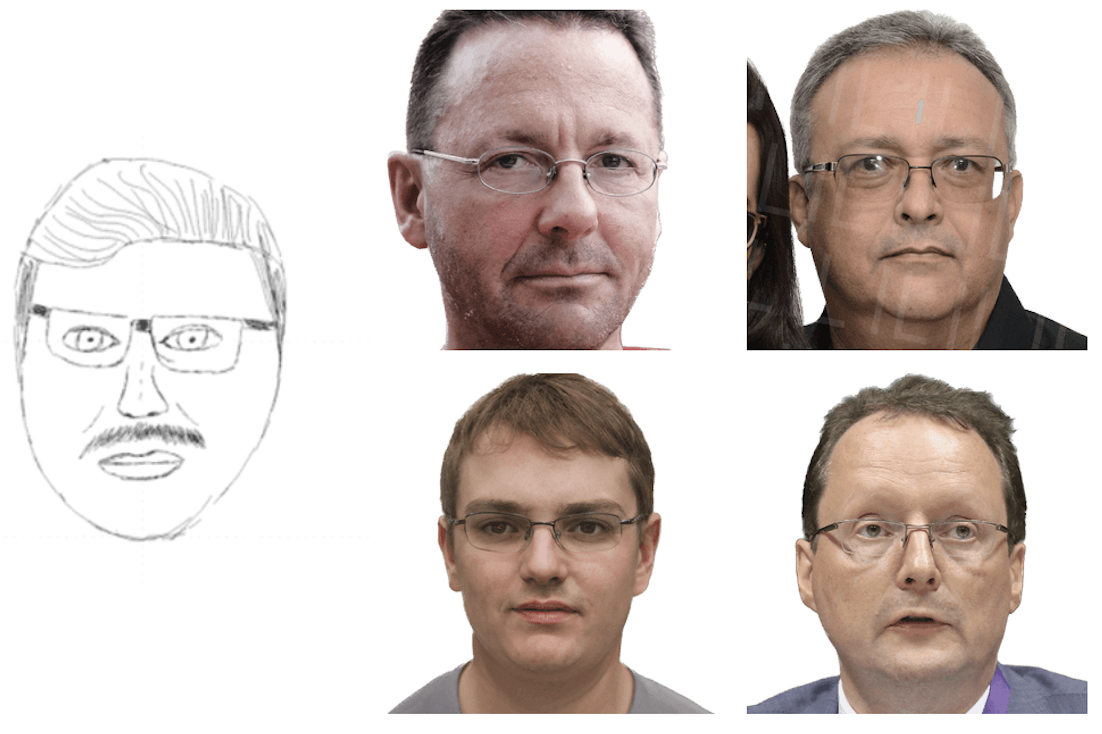
\includegraphics[width=.4\textwidth]{figures/RISULTATI/sketch0.png}} \quad
    \subfloat[][\emph{}]
    {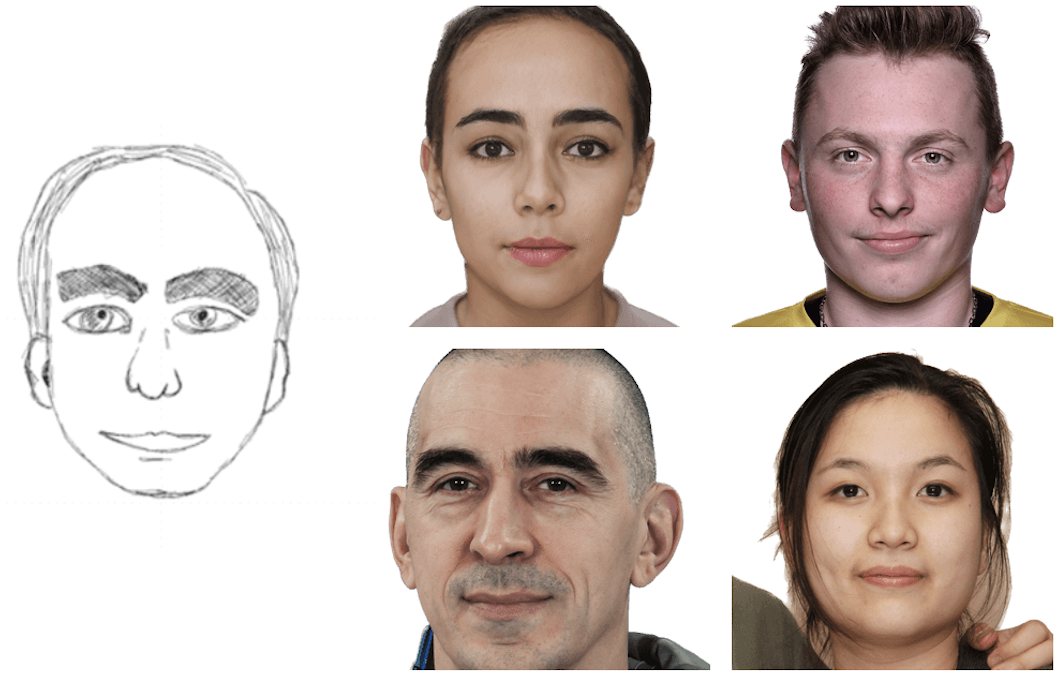
\includegraphics[width=.4\textwidth]{figures/RISULTATI/sketch2.png}}
    \caption{Images associated with sketch \num{0} and \num{2}}
    \label{fig:similar images sketch 0 and 2}
\end{figure}

\noindent An additional analysis was conducted to examine the correlation between the response time and the accuracy of the choices made. 
In particular, the Spearman correlation coefficient was used, as it measures the strength and direction of the association between two variables. Specifically, it assesses the monotonic relationship between the two variables, meaning that it measures how well the relationship between the variables can be described by a monotonic function. 

\noindent In order to determine if such correlation exists, the two variable considered are the percentage of correct responses and the average time spent to choose the response for each sketch. The Spearman correlation coefficient obtained is \num{-0.56} with a p-value of \num{0.01}, results that indicate statistically significant negative correlation between the two variables. Therefore, as the average time spent to answer increases, the number of correct responses decreases.
Figure~\ref{fig:scatter plot relation avg time and percentage of correct responses} shows this negative correlation between the average time spent per response and the percentage of correct responses. The percentage of responses is represented on the x-axis, and the time spent per response is represented on the y-axis.

\begin{figure}[!ht]
  \centering
  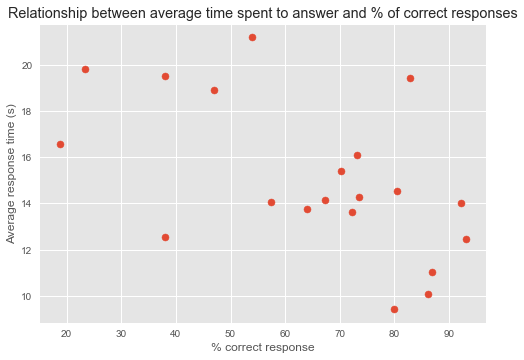
\includegraphics[width=0.8\textwidth]{figures/RISULTATI/relationshipTime-responses.png}
  \caption{Scatter plot representing the relation between the average time and the percentage of correct responses}
  \label{fig:scatter plot relation avg time and percentage of correct responses}
\end{figure}

\noindent A further test was conducted during the process of collecting sketches, mentioned earlier in this chapter, several people expressed their curiosity in testing the model's capability to generate an image of the most dreamt person in the world as claimed by many people since 2006.
The phenomenon was called “This Man” and it also has a dedicate website where people experiences are collected and shared, including the description of this man.
Given the interest and the curiosity generated, the GAN model was used to attempt to produce the image corresponding to the man sketch. By feeding the sketch of this famous man into the trained model, the objective was to generate a visual representation of this person. The resulting image is illustrated in Figure~\ref{fig:this man output}, and it reveals the face of a woman maintaining the primary facial characteristics of the original sketch.

\begin{figure}[!ht]
  \centering
  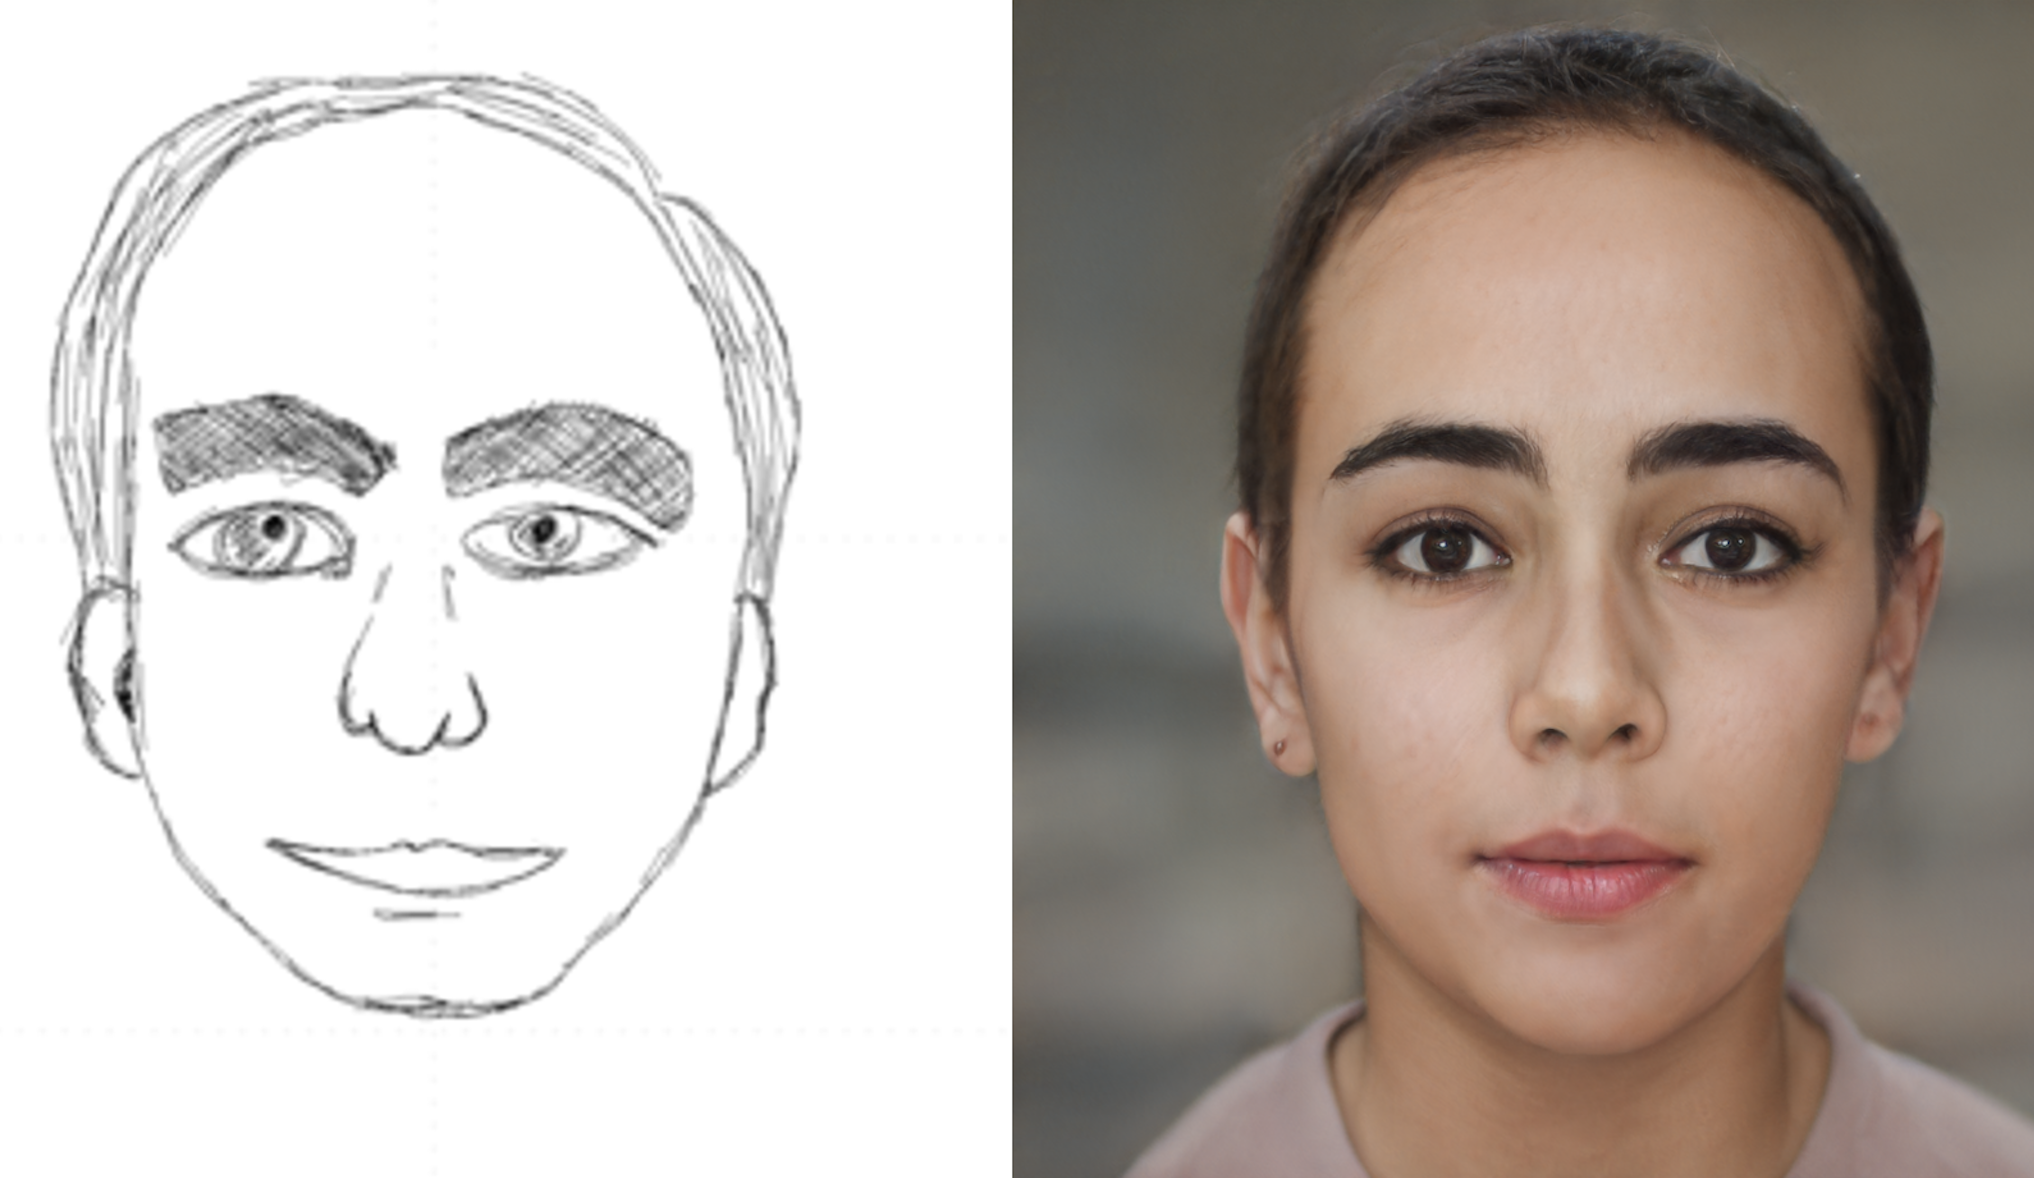
\includegraphics[width=0.8\textwidth]{figures/RISULTATI/thisMan-output.png}
  \caption{Sketch of the most dreamt man and its corresponding generated image}
  \label{fig:this man output}
\end{figure}